\documentclass[format=final, language=chinese, degree=fyp]{hustthesis}

\usepackage[colorinlistoftodos,prependcaption]{todonotes}
\usepackage{enumitem}
\usepackage{listings}
\usepackage[section]{placeins}
\usepackage{graphicx}
\usepackage{subcaption}

\stuno{U201315168}
\schoolcode{10487}
\title{基于Android平台的网络防火墙的设计与实现}{An Implementation of Android Firewall}
\author{易亚洲}{Yazhou Yi}
\major{信息安全}{Information Security}
\supervisor{李平}{Ping Li}
\date{2017}{6}{10}

\zhabstract{
	本文从需求分析出发,对实现一款Android网络防火墙应用进行了模块分析,提出了一种实现Android网络防火墙应用的架构,并对这个实现的应用进行了兼容性,功能和性能三方面的评估测试,最后证明该实现方式的正确性和可行性。
}

\zhkeywords{防火墙, 安卓, 网络, 安全}

\enabstract{
Based on the analysis of needs, this paper analyzes the application of an Android network firewall, and puts forward a framework to realize the application of Android network firewall, and has carried on the compatibility test, the function and the performance evaluation , and finally prove the correctness and feasibility of the implementation.
}

\enkeywords{Firewall, Android, Network, Security}

\graphicspath{ {images/} }

\begin{document}

\frontmatter
\maketitle
\makeabstract
\tableofcontents
\listoffigures
\listoftables
\mainmatter

\chapter{绪论}\label{chapter:1}
\section{项目背景}

\subsection{Android系统}
Android是由Google开发的一个基于Linux内核的开源操作系统,目前主要应用于手机,平板电脑,电视,车载电脑等移动设备,。Android大部分代码使用Apache 2.0协议开源,使得各大厂商都可以基于Android系统进行二次开发,打造出多种多样的Android系统,例如小米公司的MIUI,华为EmotionUI等,这些Android系统的各种深度定制版给了用户很多种选择。

Android操作系统在智能手机的市场份额自从发布以来一直保持持续上升。
在推出后两年,即2010年末,市场占有率超越塞班系统,成为全球第一大智能手机操作系统,
2016年第三季度最新数据显示,Android市场份额已经达到了86.8\%,远远超过其他操作系统的总量,并且份额将会长期保持。不像iOS操作系统,Android每年都有数以百计的合作厂商发布大量新的机型,例如Oppo,三星,华为等,用户有着大量的选择。
Android操作系统本身开源的特性和在智能手机市场上的火热,让Android系统的生态系统极度丰富。同样是Android系统,不同公司定制的版本往往有着不一样的交互界面,也有着不同的自带应用。Android用户可以在应用市场选择下载数以百万计的App。但这也带来了碎片化的问题,在系统版本上,Android发布的新版本难以快速普及,大量用户仍然使用陈旧的版本,截止2016年末,接近50\%的用户仍然在使用2014年和更久以前发布的版本。这不仅给开发者带来了兼容性上的困难,也导致了巨大的安全隐患:旧版本用户系统上的安全漏洞得不到修复,新的安全机制无法生效。同时,各种定制Android的厂商的技术实力参差不齐,存在很多粗制滥造的二次开发版本,其安全性得不到任何保障。


\section{研究意义}

随着智能手机的普及,以及4G网络的快速发展,越来越多的用户开始使用手机上网冲浪。中国互联网络信息中心(CNNIC)发布了第38次《中国互联网络发展状况统计报告》。《报告》显示,截至2016年6月,中国网民规模达7.10亿,其中手机网民规模达6.56亿,占比达92.5\%。中国各类第三方市场鱼龙混杂,管理混乱,对应用上架的审核存在不规范,不严格甚至完全没有审核的现象。

根据赛门铁克(Symantec)最新互联网安全威胁报告称,在所有的安卓应用程序中有17\%是恶意软件,如autoref{fig:2}。尤其是Google Play市场无法提供服务的地区,用户不得不从未知来源下载安全应用,各种第三方市场鱼龙混杂,其中有很多恶意软件混迹其中,也有很多安全性低容易收到攻击的应用。

\begin{figure}[h!]
\centering
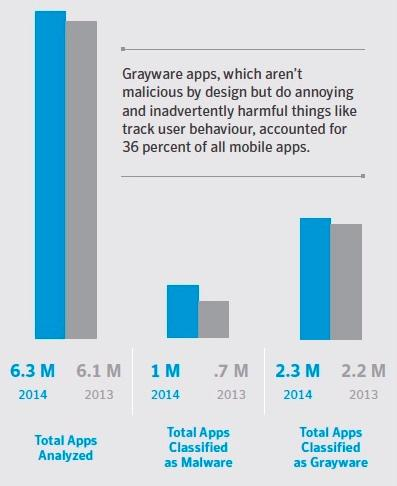
\includegraphics[width=.4\textwidth]{symantec_report}
\caption{Symantec恶意软件数量报告}\label{fig:2}
\end{figure}

腾讯移动安全实验室发布了2016年手机安全报告,报告显示2016年Android病毒包共增加2341.8万,同比增长40.20\%。2016年Android手机病毒感染用户数同比增长62.43\%,感染用户数总量达到5亿人次,达到历年新高。其中资费消耗类占比高达84.24\%,在2016年手机病毒类型中排名第一。
资费消耗类的病毒是指的在未经用户授权的情况下,通过频繁连接网络、发送短信等方式,导致用户资费损失。这部分病毒往往帮助一些广告商提高App装机量或点击率进行恶意推广,不断联网下载,消耗用户流量。

针对资源消耗类病毒,网络防火墙可以启动有效的防范和遏制的作用,将不可信应用的网络权限进行限制,对可疑应用的数据通信进行监控,是遏制这类病毒的最重要手段。此外,对于远程控制、隐私窃取等类型的软件,限制网络通信也是有效可行的重要举措。

Android系统自带的通信权限管理仅仅允许对特定应用设置是否允许链接网络,无法对Wifi网络和蜂窝数据网络区分设置,也不支持多种条件下的自定义规则,如灭屏和亮屏,特定网络,限制时段等条件,而且,不支持按协议过滤,按源目的地址过滤等基本防火墙功能。所以我们有必要开发一款Android网络防火墙来完善这些功能,满足用户对Android网络管理更高级的需求。
所以在目前Android用户数量持续增长,资费消耗病毒日渐猖獗,而Android系统网络功能不全的情况下,所以我们提出了设计并实现一个基于Android平台的网络防火墙的课题,旨在通过对Android系统网络通信的监控和管理的实现,研究Android网络安全,设计一个可用的Android网络防火墙,改善Android系统的安全性。

\section{预期目标}

本论文的目标是通过设计和实现一个Android网络防火墙,通过对Android系统网络通信的监控和管理,提高Android系统的安全性,有效防范资费消耗类恶意软件。目前存在多种Android防火墙的实现方案,但我们希望避提供一个普通Android用户下载安装后即可用的解决方案,而不是要求提取系统Root权限,甚至定制操作系统内核等难以实行的方案。本文采取的设计方案不是类似传统防火墙由管理员设定一组规则然后一直照此执行直到修改规则,而是采用交互式规则,在应用尝试进行一些网络请求时,通知用户做出决策:允许或者拒绝,并且即时的更新规则。同时需要监控连接的流量消耗,提供地址的相关信息,为用户做出决策提供帮助。


最后,将针对防火墙的性能,对处理每个包时引入的能耗,包丢失和延迟进行基准测试。通过分析证明,使用这样的防火墙是可行的,并且不影响Android设备的日常功能。

\section{需求分析}

在对市场上多款防火墙类应用软件进行分析和比较之后,将用户需求列为以下几点:
\begin{itemize}
	\item 过滤Android系统所有流量\label{item:1}
	\item 支持多样的防火墙规则,如规则支持WiFi和数据流量状态、亮灭屏状态等
	\item 支持文件系统敏感区域病毒监控
	\item 支持恶意网页拦截
	\item 图形界面,操作简便,通俗易懂
\end{itemize}

对于上述需求,进行明确和细化,方便开发和测试验收:
\subsection{基础要求}

\subsubsection{兼容性要求}
	在兼容性方面,我们需要做的包括系统版本兼容、CPU架构兼容,权限兼容和屏幕尺寸兼容。在此提出具体的兼容要求:

\begin{itemize}
	\item 兼容Android 4.0及以上系统,能在这些版本的Android系统上正常运行
	\item 兼容ARM,x86和x86\_64架构,能在这些架构的手机上正常运行
	\item 支持多种版本Android系统的权限系统
	\item 能在1280*720至2560x1440多种分辨率的手机上正常显示
\end{itemize}

\subsubsection{易用性要求}
	作为一款移动应用软件,提供良好的易用性是必要的,我们提出了以下要求:
	\begin{itemize}
		\item 提供良好的GUI以及良好的交互
		\item 提供快捷切换的开关
		\item 提供友好的通知和提醒
	\end{itemize}

\subsection{功能要求}

\subsubsection{防火墙功能}
\begin{enumerate}
	\item 交互式规则:如果新建立的连接没有已知的规则进行决策,会通知用户即时作出决策。在用户可以在弹出的通知栏里选择允许或者拒绝,然后就会记住该规则,在以后有相同的连接时采用该规则;如果用户选择了拒绝,该连接将会被切断。
	\item 审计式规则:用户可以查看近期所有的连接记录,可以选择对特定连接快捷建立规则
	\item 规则的适用范围:
		\begin{itemize}
			\item 面向应用:用户可以设定规则只对特定应用生效
			\item 面向出口:用户可以设定规则只对特定网络环境生效,如Wifi/2G/3G/LTE/漫游
			\item 面向特定状态:用户可以设定规则只对特定手机状态生效
		\end{itemize}
	\item 防火墙默认策略:当用户没有为特定应用设定规则时,采用默认策略
	\item 实时网速监控:用户可以在通知栏查看实时的网速
	\item 新应用提示:在用户安装新的应用程序后,会提示用户为其创建规则
\end{enumerate}

\subsubsection{文件防护功能}

文件防护功能监控文件系统的关键区域,对潜在的威胁进行扫描,其功能的要求如下:
\begin{itemize}
	\item 扫描文件病毒
	\item 监控下载文件夹自动扫描可疑文件
	\item 自定义监控的文件位置
\end{itemize}


\subsubsection{网页防护功能}

网页防护功能主要提供对存在威胁的网站的屏蔽,该功能主要基于防火墙功能实现,要求较为简单:能对存在威胁的网站进行屏蔽。

\subsection{性能要求}

网络防火墙为了提供额外的安全保障,必须尽可能的持续运行。所以网络防火墙必须对Android移动设备的的性能和电量的消耗保持在最小。所以必须采取措施将防火墙规则匹配的耗时和对包处理的耗时降到最低,例如TCP连接可以只对SYN和FIN包进行处理便可实现监控TCP连接的生命周期,此外我们还需对其他协议及在所有可能的环节降低性能损失,并通过性能测试和报告证明防火墙对设备所造成的性能损失在可以容忍的较小范围之内。

\subsection{可选高级功能要求}

为了提高体验和方便实际使用,还可实现一些非核心功能的特性:
\begin{enumerate}
	\item (可选)提供一定的交互动画
	\item 日志查看:记录应用程序的网络访问尝试
	\item 支持系统应用:支持对系统应用设置规则
	\item 支持IPv6:提供对IPv6及ICMPv6的支持
	\item 端口转发:支持增加/删除/编辑端口转发规则
	\item 配置导入导出:支持将规则和配置导出到文件或者从文件中导入
	\item 持久有效:防火墙必须持续有效的工作:
		\begin{itemize}
			\item 进程必须尽可能避免被系统停止或杀死
			\item 防火墙必须在断开时尝试重新启动
			\item 防火墙必须在开机自动启动
		\end{itemize}
\end{enumerate}


\section{章节介绍}

本文一共六章,第一章讲述项目背景和研究意义,然后对网络防火墙应用进行了需求分析。紧接着,第二章阐述项目的理论基础,这包括Android系统原理和Android防火墙的实现思路,并介绍了Android开发工具。第三章则对应用的设计进行了概要设计,这一章主要针对第一章中提出的需求分析给出了功能设计,划分了应用的功能模块,也对应用的UI设计进行说明。第四章则对实现各个功能模块进行了详细说明,先是对三个功能分别进行了设计,描述了详细的架构设计和实现方式,然后对模块公用的数据库持久化和非数据库持久化方案进行的描述,最后阐述了如何解决应用的兼容性问题。第五章对完成的网络防火墙进行了兼容性,功能,性能三个方面的测试,证明了本文提出的实现方案的可行性和可用性。最后第六章对本文内容进行了总结,也对Android网络防火墙的发展和应用进行了展望。

\chapter{设计原理}\label{chapter:3}

\section{Android系统架构}

Android操作系统的核心是Linux内核的一个分支,但也有很多的修改和扩充。其中主要包括:去除了X Windows System,不支持GNU库。另外主要增加了两个部分,Binder IPC和Wakelock管理。

Android系统的架构如图所示,分为四层,自上而下分别是应用程序(Applications),应用程序框架(Application Frameworks),系统运行库与Android运行环境(Libraries \& Android Runtime),Linux内核(Linux Kernel)。
\begin{itemize}
	\item 应用程序层由各种应用软件组成,如短信,浏览器,地图等,这些应用可以是系统自带,也可以是从应用市场下载。
	\item 应用程序框架层提供了应用程序运行需要的各种API和系统服务,主要由Java编写。开发者开发Android应用需要对这一层由较多的了解。它提供了用于实现图形界面的视图,活动管理器,窗口管理器,内容提供者,资源管理器,通知管理器,包管理器,等。
	\item Android运行库是为Android系统中各种组建运行而提供的C/C++库的合集,用以实现底层的图形绘制,媒体播放录制,Web页面渲染,3G图形,SQLite数据库等功能。而Android运行时则是Android虚拟机的实现,Android 5.0以前是Dalvik虚拟机,5.0以后是ART虚拟机,用以执行应用软件中的字节码。
	\item Linux内核为Android提供硬件驱动,内存管理,进程眼里,网络协议栈和安全体系等实现。同时,Android加入了针对移动设备优化的电源管理和Binder机IPC机制。
\end{itemize}

\section{Android防火墙}
实现Android防火墙,实现对流量的过滤,有多种实现方式,Android内核是linux内核的一种分支,也提供netfilter和iptable,可以参考Linux内核防火墙的实现方式实现Android防火墙。

\subsection{Netfilter防火墙}

Netfilter是Linux 2.4.x之后版本提供的包过滤的框架,它在TCP/IP协议栈中提供了相应的Hook,允许我们对网络数据包进行过滤,丢弃,修改等操作。通过netfilter中的一些函数即可实现防火墙应用。而iptables是linux提供的一个基于netfilter工具,使用户可以对整个操作系统收发的数据包就行拦截修改拒绝等操作。
以IPv4为例,netfilter在IPv4协议栈中定义了五个hook,在这五个点使用nf\_hook\_ops结构注册hook,过滤经过该点的所有包,nf\_hook\_ops定义如下:

\begin{lstlisting}[language=c]
struct nf_hook_ops
{
    struct list_head list;
    nf_hookfn *hook;
    int pf;
    int hooknum;
    int priority;
};
\end{lstlisting}

nf\_hook\_ops中的nf\_hookfn就是hook函数,实现一个nf\_hookfn函数,在该函数中实现对包的读取解析并过滤,返回NF\_ACCEP,NF\_DROP等返回值,即可实现对数据包的操作。

\subsection{VPN防火墙}

Android系统本身提供了制作VPN应用的API,允许第三方应用向系统提供VPN,系统负责将网络流量转发到VPN应用,VPN应用可以建立隧道实现VPN服务。而在这个过程中,VPN应用可以对网络流量进行分析和过滤,实现防火墙的功能。

\subsection{方案对比}
netfilter/iptable需要调用netfilter api或执行iptable,这都必须拥有root权限才有可能实现。Root本身就是利用漏洞才得以实现的,并且root之后的手机毫无安全性可言,与我们做防火墙提高安全性的初衷相悖。

VPN方案由于使用了Android官方提供的公开API,可以不需要Root权限运行,只需要用户在第一次启动VPN时授予许可,也没有给系统带来额外的安全风险。其缺陷在于VPN服务只允许启动一个,将会导致用户使用防火墙后无法使用其他VPN。

以加强Android安全作为出发点,通过对两种方案的对比,我们最后决定采用VPN方案实现Android防火墙。

\section{Android开发工具}

Google为开发Android应用程序提供了一系列的开发工具。

\begin{itemize}
	\item Android SDK: Google提供的Android开发套件
	\item Android Studio: 用来开发Android的集成开发环境
	\item Android Emulator: 用来测试的Android虚拟机
	\item Android NDK: Android Native开发
	\item Android Debug Bridge: Android调试
\end{itemize}


\section{Android信息传递机制}

\subsection{Intent信息传递}

Intent是Android中独有的一种实现交互与通讯的机制。Intent不仅广泛应用于应用程序内部各种组件(如不同界面之间,界面和后台服务之间)彼此交流,而且在应用与应用,应用与系统之间的事件传递中也广泛使用。Intent可以包含应用程序的一次行为的动作(action),种类(category),标志(flag)和附加数据(extra)。

如下代码,实现了在主界面中向后台服务发送了一个Intent,该Intent的包含了附加数据"start"命令,让后台服务启动VPN:

\begin{lstlisting}[language=java]
	// 创建intent对象
    Intent intent = new Intent(this, ServiceSinkhole.class);
 	// 在intent对象中放入指令
    intent.putExtra(EXTRA_COMMAND, Command.start);
    startService(intent);
\end{lstlisting}

系统在接收到上述操作后,会回调后台服务的相应代码处理该Intent:
\begin{lstlisting}[language=java]
    @Override
    public int onStartCommand(Intent intent, int flags, int startId) {
        // 获取intent中的指令
        if (intent != null && intent.hasExtra(EXTRA_COMMAND) &&
                intent.getSerializableExtra(EXTRA_COMMAND) == Command.start) {
            start();
        }
\end{lstlisting}

\subsection{本地广播通知}

本地广播(Local Broadcast)是一种进程内的事件监听机制。进程内任何时刻均可注册任意事件监听器;当某一事件发生时,就会通知所有监听该事件的监听器。通过如下代码,可以监听ACTION\_SCAN事件:


\begin{lstlisting}[language=java]
LocalBroadcastManager.getInstance(FileScannerService.this).registerReceiver(mReceiver, new IntentFilter(DownloadFileObserver.ACTION_SCAN));
\end{lstlisting}
 

在需要的时候需要反注册监听器,如下:
\begin{lstlisting}[language=java]
LocalBroadcastManager.getInstance(FileScannerService.this).unregisterReceiver(mReceiver);
\end{lstlisting}

\chapter{概要设计}

\section{功能设计}

我们设计的网络防火墙需要在网络方面提供全方面的网络防护。首先,需要实现传统PC防火墙拥有的网络流量防护,同时针对移动网络环境,提供面向移动应用和面向移动网络环境的优化;其次还需要针对下载操作提供加强,实现对下载文件的监控扫描;最后,还需要实现对网页安全的防护,实现对不安全网站的屏蔽。根据这些设计概念,我们将整个应用设计成了三个大模块,如\autoref{fig:3-0}。

\begin{figure}[!h]
\centering
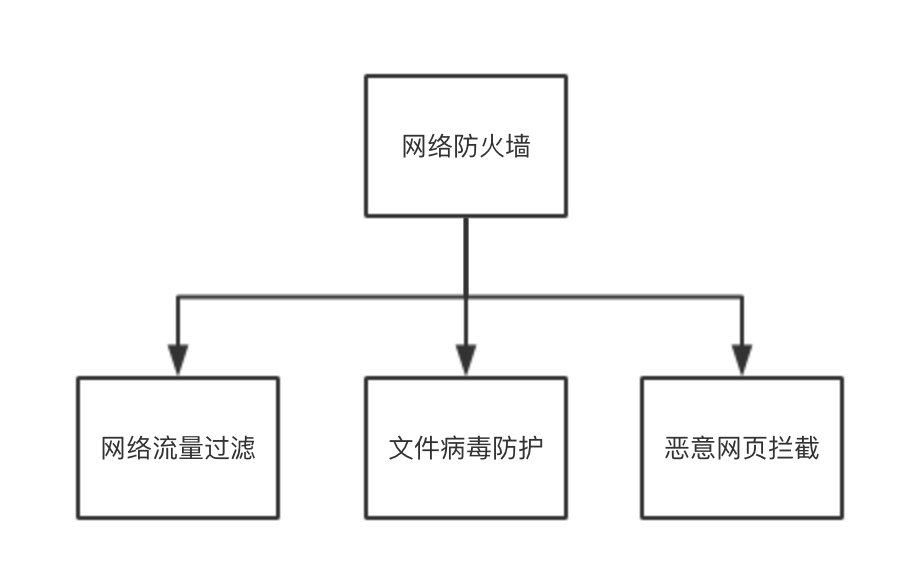
\includegraphics[width=0.8\textwidth]{function_all.png}
\caption{总体功能模块图}\label{fig:3-0}
\end{figure}


下面我们分别对这三个模块进行需求分析和功能设计。

\subsection{网络防护}

网络防护旨在提供传统防火墙的网络连接的管理功能,同时针对移动网络环境,提供面向移动应用和面向移动网络环境的优化。

用户期望一个Android防火墙应用提供友好的交互界面和正常的拦截效果。设计中应实现:
\begin{itemize}
    \item 拦截管理界面:对某个应用设置是否拦截流量
    \item 全局控制开关:切换全局防火墙状态
    \item 查看历史通信日志:查看单个应用的通信日志,包括尝试访问的地址,端口,协议类型,
    \item 设置亮屏等特殊请客的规则
    \item 支持IPv6
    \item 支持家庭网络,按流量计费网络等单独规则
    \item 配置导出导入
\end{itemize}

根据上面的需求分析,设计了如\autoref{fig:3-1}的功能模块。
\begin{figure}[!h]
	\centering
	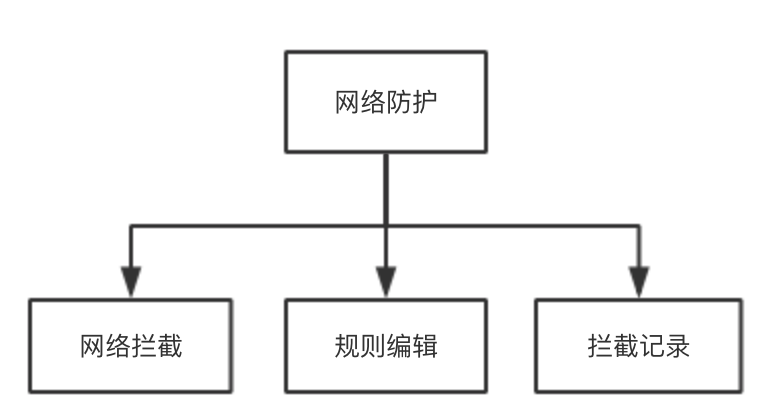
\includegraphics[width=0.8\textwidth]{function_1.png}
	\caption{网络防护功能模块图}\label{fig:3-1}
\end{figure}

图中功能模块将网络防护划分为4个子模块,分别为网络拦截、规则编辑和拦截记录。

\subsection{文件防护}

文件防护旨在提供本地文件的病毒扫描以及实时文件系统监控扫描的功能。这个功能核心在于对下载文件夹等敏感目录进行监控,自动的进行恶意软件扫描和警报,另外也提供了让用户自定义扫描任何位置的功能。

\begin{itemize}
    \item 实时监控控制开关:关闭和启用实时文件病毒防护
    \item 实时监控配置界面:允许用户添加和删除监控区域
    \item 自定义扫描:用户选取特定扫描区域进行扫描
    \item 最近扫描记录列表:用户在此查看所有的扫描记录和扫描结果
    \item 威胁处理界面:用户对识别出的威胁做出处理
\end{itemize}

根据上面的需求分析,设计了如\autoref{fig:3-2}的功能模块。
\begin{figure}[!h]
	\centering
	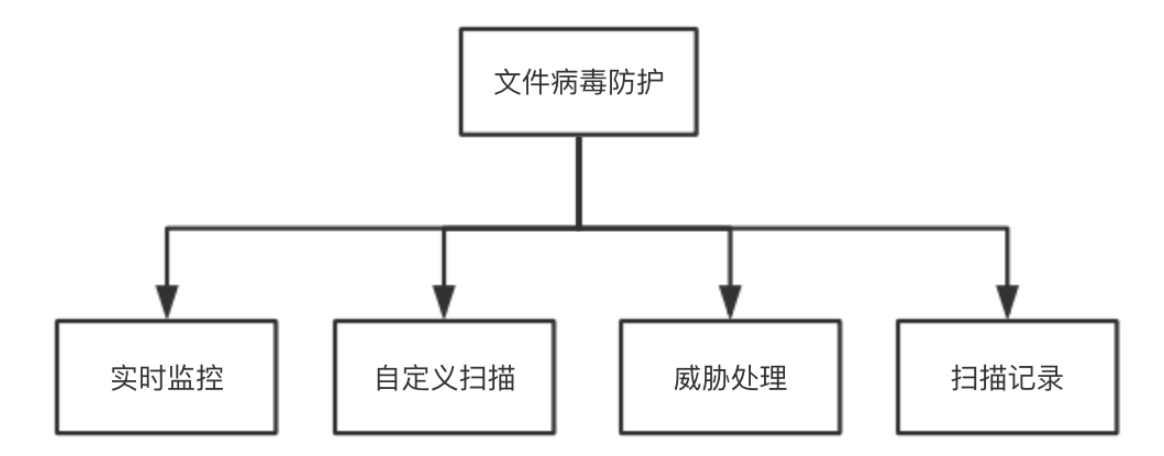
\includegraphics[width=0.8\textwidth]{function_2.png}
	\caption{文件防护功能模块图}\label{fig:3-2}
\end{figure}

图中功能模块将文件病毒防护划分为4个子模块,分别为实时监控、自定义扫描、威胁处理和扫描记录。


\FloatBarrier
\subsection{网页防护}

网页防护通过对流量的过滤,将存在威胁的ip以及存在恶意代码的网页进行屏蔽,阻止这些网站威胁到手机安全。在是实现上,以全局代理作为基础,对流量数据进行过滤,针对http和https等协议进行额外的检查。为了进行检查,首先需要一个恶意网站网址和恶意ip的列表,这种列表存在多种机构在各自独立的维护,主要是url reputation相关。在我们的安全软件上,需要下载一份列表,并定期进行更新,在发生网页访问时,通过Url从本地的列表查询是否是记录在案的恶意网站。对于恶意网站,忽略这个网络请求,并返回一个虚构的对用户进行恶意网站提示的网页,这个网页在软件本地生存。

\begin{itemize}
    \item 网页拦截:实现对网页的拦截,能够对功能进行开关
    \item 拦截记录:能够显示拦截记录,将历史屏蔽的记录进行显示
    \item 本地数据更新管理:能够控制本地黑民单的更新
    \item 白名单管理:增加网页白名单
\end{itemize}

根据上面的需求分析,设计了如\autoref{fig:3-3}的功能模块。
\begin{figure}[!h]
	\centering
	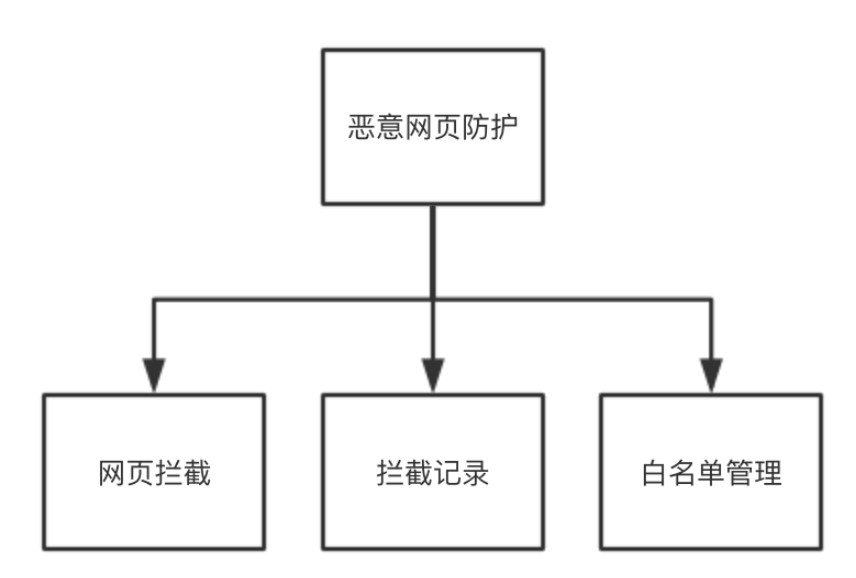
\includegraphics[width=0.3\textwidth]{function_3.png}
	\caption{网页防护功能模块图}\label{fig:3-3}
\end{figure}

\section{UI设计}

为了给用户提供简便的操作和管理方式,我们对应用设计了符合Android设计规范的图形界面,主要UI设计如下:

\subsection{导航页}

导航页是应用程序的入口,用户打开程序首先看到的就是这个页面。这个页面较为简单,列举了三个主要功能,分别是网络防护,文件防护和网页防护。用户点击这三大板块即可进入任一主功能的页面。如如\autoref{fig:3-2-0}所示。

\begin{figure}[!h]
	\centering
	\includegraphics[width=0.3\textwidth]{3-2-0.png}
	\caption{导航页UI图}\label{fig:3-2-0}
\end{figure}

\subsection{网络防护界面}

网络防护界面是用户管理网络防护的控制台。最顶部的工具栏,工具栏下方是应用列表,两者中间可以插入通知消息;在整个页面的右下角有一个悬浮按钮,这个是网络防护的总开关。如\autoref{fig:3-2-1}所示。

\begin{figure}[!h]
	\centering
	\includegraphics[width=0.3\textwidth]{3-2-1.png}
	\caption{网络防护UI图}\label{fig:3-2-1}
\end{figure}

\begin{itemize}
    \item 工具栏包含搜索及排序按钮,以及最右边的菜单按钮,菜单按钮可打开设置界面、帮助界面和关于等界面。
    \item 应用列表列出了所有的用户程序,并在每个用户程序旁边提供了两个按钮,分别对该应用所有的Wifi,数据流量的通信进行拦截
    \item 通知消息栏在没有消息时会隐藏,需要时会提示重要信息,比如当前状态或者异常信息
    \item 悬浮总开关是全局防火墙开关,用于控制VPN是否启用
\end{itemize}

应用列表只提供了两个按钮供用户快捷配置,但用户如果需要想要进行更高级的配置,点击列表项即可打开高级配置:

用户可以设置亮屏或漫游时的白名单,也可将规则恢复为默认行为,还可以查看该应用程序所有尝试的访问请求记录,包括时间,地址或域名,协议类型和端口,对于每一条记录,可以单击设置对该记录选择:屏蔽或允许类似的请求,或者访问/whois该连接。



\subsection{文件防护和网页防护}

文件防护界面是用户管理文件防护的控制台。由置顶的状态栏,通知列表和悬浮开关组成。如\autoref{fig:3-2-2}所示。
网页防护较为简单,由启用开关,更新规则按钮等组成。

\begin{figure}[!h]
	\centering
	\includegraphics[width=0.3\textwidth]{3-2-2.png}
	\caption{文件防护UI图}\label{fig:3-2-2}
\end{figure}

\subsection{设置,日志,帮助和关于界面}
设置界面采用了Android规范的列表形式,选择列表项可进入二级设置界面。
另外还有日志界面显示全局日志输出,帮助界面提供用户操作上的指导和关于界面展示开发者信息及反馈方式。

\chapter{详细设计}

\section{网络防护模块}

根据实现防火墙的原理和功能需求,设计了成如\autoref{fig:5}的应用架构。

\begin{figure}[!h]
\centering
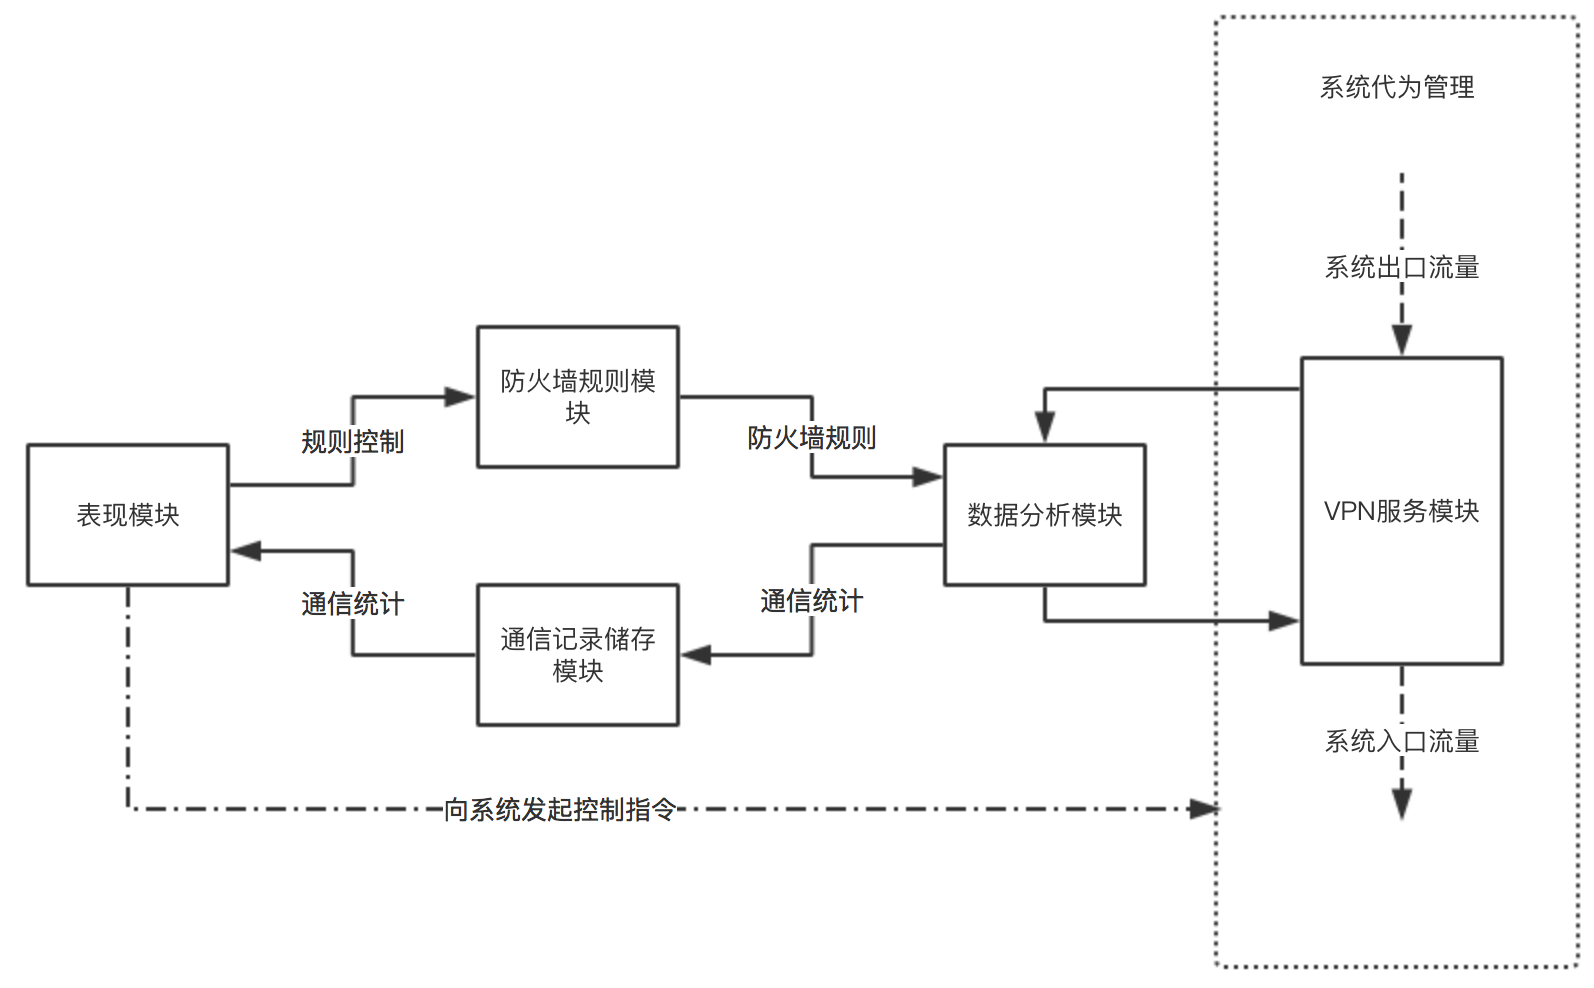
\includegraphics[width=1\textwidth]{function_1_ori.png}
\caption{网络防护架构图}\label{fig:5}
\end{figure}

上图中将网络防护模块分成了5个逻辑模块进行实现。其需要实现的基本功能如下:

\begin{itemize}
	\item 表现模块\\ 表现模块采用Activity作为主要实现,为用户提供友好的图形界面,是用户操作和管理防火墙的门户,是所有功能的入口,同时也承担着,在VPN服务层返回相应的信息(比如要求用户对是否允许某个应用的连接进行选择)时,对用户进行提醒;
	\item VPN服务模块\\该模块是继承并实现Android提供的VpnService的关键组件,用以实现VPN的功能,将VPN过滤的流量传递到下一层进行解析,并根据解析和匹配的结果,向系统回应是否作相应的处理;
	\item 数据分析模块\\该模块主要完成将网络数据包进行解析,从中提取协议、地址、会话时间等关键信息,并用防火墙规则进行匹配,判断数据包是否放行;
	\item 防火墙规则模块\\该模块负责持久化储存防火墙规则数据,将防火墙规则抽象成相应的Java对象,供数据包分析模块使用;同时,由于在大量数据包中,规则的读取极其频繁,防火墙规则模块也负责实现对规则的缓存,提高性能;
	\item 通信记录储存模块\\主要负责为通信记录提供持久化储存。
\end{itemize}

\subsection{VPN服务模块}

\subsubsection{VPNService启动过程}

VPN服务模块是通过继承实现Android提供的VpnService类来实现的。VpnService是用来继承并实现自己的VPN应用的基础类。它创建了虚拟网络接口,配置地址和路由规则,返回一个文件描述符给应用。对文件描述符每一次读,就会读取一个通过这个接口向外发出的数据包;对文件描述符的每一次写,就会插入一个入数据包,对接口而言,就相当于这个接口接收到了这个数据包。这个虚拟网络接口运行于IP协议层,所以数据包的 开头都是IP数据头。通过这个API,应用可以实现在隧道中与远程服务器的数据包处理和交换,构造一个VPN应用。

允许应用拦截数据包带来了巨大的安全隐患。一个VPN应用可以轻而易举的切断网络,此外多个VPN应用也可能互相冲突。系统采取了多种措施来解决这个问题。主要是:
\begin{enumerate}
 	\item 第一次创建VPN链接的时候,必须需要用户的授权;\label{item:1}
	\item 同时只能有一个VPN运行。如果创建一个新的连接,现有的连接都会被切断;
	\item 在VPN运行的全程,都会有一个系统级的通知显示在通知栏告知用户;
	\item 系统会提供一个系统级的对话框,告知用户当前VPN连接的信息并允许用户断开VPN连接;
	\item 当文件描述符关闭的时候或VPN应用崩溃和被系统杀死的时候,网络状态会被自动还原。
\end{enumerate}


VpnService中有两个重要方法:

\begin{lstlisting}[language=Java]
prepare(Context);
establist();
\end{lstlisting}

前者处理用户的行为和停止其他应用的VPN连接,后者通过VpnService.Builder提供的参数创建VPN连接。应用必须调用 prepare(Context)确保取得对当前类其他方法的授权。这个授权随时可能被收回。创建一个VPN连接的步骤如下:
 \begin{enumerate}
     \item 当用户按下连接的按钮时,调用prepare(Context),并且在这个方法返回的intent非空时启动这个intent;这个方法为了取得用户的授权,这个方法返回null时说明用户此前已经授权过;
     \item 当用户授权之后,启动VpnService服务;
     \item 创建一个到远程服务的隧道,并且交换vpn连接的参数并配置好;
     \item 将这些参数应用到 VpnService.Builder , 并通过调用establish()创建VPN接口;
     \item 在隧道和返回的文件描述符之间处理和交换信息;
     \item 当onRevoke()收回权限时,关闭文件描述符和隧道。
\end{enumerate}

VPNService的启动过程如\autoref{fig:4-1-1}所示,当用户通过UI界面启动VPN时,会触发该过程,如果该过程执行到启动数据分析模块,会调用native代码启动一个新线程,该线程运行数据分析模块,数据分析模块负责对文件描述符读写数据,实现VPN的功能。数据分析模块的逻辑我们会在下一节中进行介绍。

	\begin{figure}[h]
		\centering
		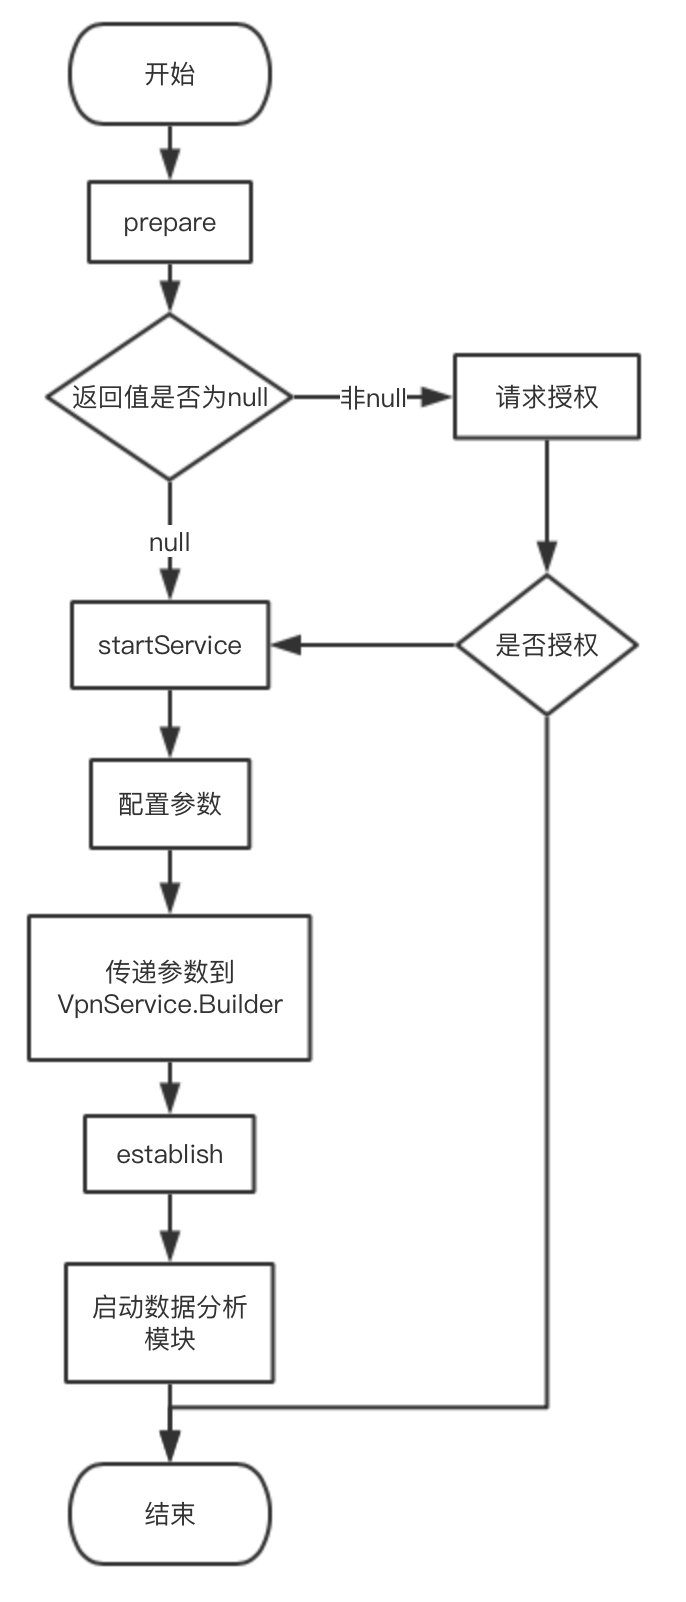
\includegraphics[width=0.6\textwidth]{process_4_1_vpn.png}
		\caption{VPNService启动流程图}\label{fig:4-1-1}
	\end{figure}

 应用在继承VpnService实现VPN必须声明相应的权限和intent过滤器,范例如下:
\begin{lstlisting}[language=xml]
  <service android:name=".ExampleVpnService"
          android:permission="android.permission.BIND_VPN_SERVICE">
      <intent-filter>
          <action android:name="android.net.VpnService"/>
      </intent-filter>
  </service>
\end{lstlisting}
\FloatBarrier
\subsubsection{VPNService与UI的通信}

VpnService和Activity之前通过Intent传递信息,实现控制。如\autoref{fig:4-2-1}。

\begin{figure}[h]
	\centering
	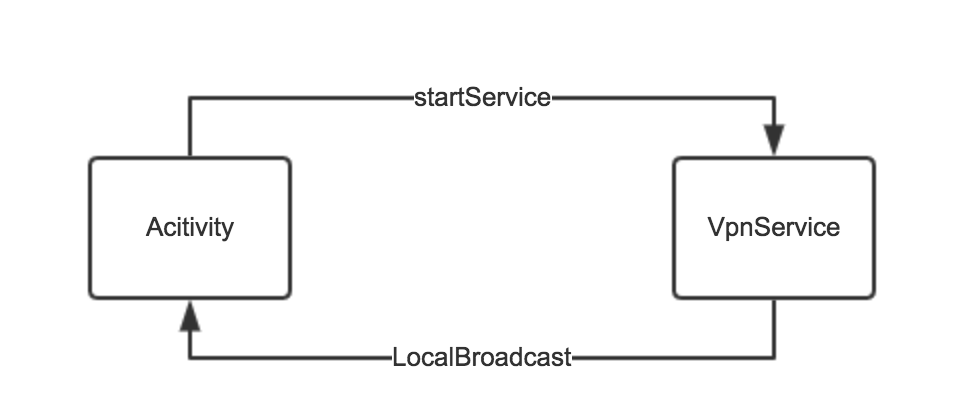
\includegraphics[width=.8\textwidth]{image_intent_commuciate.png}
	\caption{VpnService与Activity通信图}\label{fig:4-2-1}
\end{figure}

Activity是界面,VpnService是后台服务。VpnService在工作时,Activity可能并不存在,如果需要传递信息给Activity,在其不存在时,就应该忽略这条信息;而Activity运行时,调用VpnService时,如果VpnService尚未运行,则需要创建VpnService。因此才采用了不同的通信机制:
Activity注册本地本地广播接收器,VpnService通过sendBroadcast(Intent)方法发送本地广播,如果Activity存在并且正在监听,则会收到信息;
Activity通过调用startService(Intent)发送Intent到VpnService,如果VpnService没有启动则会启动,已经启动则会通知现有的Service。

Intent中可以携带信息,通过实现预定好的协议,可以从Intent携带的信息中得知命令。我们约定协议如下:
\begin{itemize}
    \item run     启动VPN后台服务,并进行请求权限等准备工作,进入就绪状态
    \item start   建立VPN连接,开启防火墙
    \item reload  重新载入防火墙配置
    \item stop    断开VPN连接,暂停防火墙,回到就绪状态
    \item stats   诊断状态,使防火墙将自身状态和日志输出到控制台
\end{itemize}

\subsubsection{VpnService状态机}

实现VpnService代码量较多,为了使逻辑清晰,采用状态机的设计。包含以下状态:
\begin{itemize}
    \item none          未就绪状态,VpnService不可用
    \item waiting       等待状态,用户已经许可了权限,但并没建立VPN连接
    \item enforcing     启用状态,VPN连接已建立,VPN正在运行
    \item stats         报告状态,VpnService需要报告当前信息,用于诊断
\end{itemize}

这些状态在使用run, start, reload, stop, stats这些命令时会发生状态迁移,状态迁移图如\autoref{fig:3} 所示。

\begin{figure}[h!]
\centering
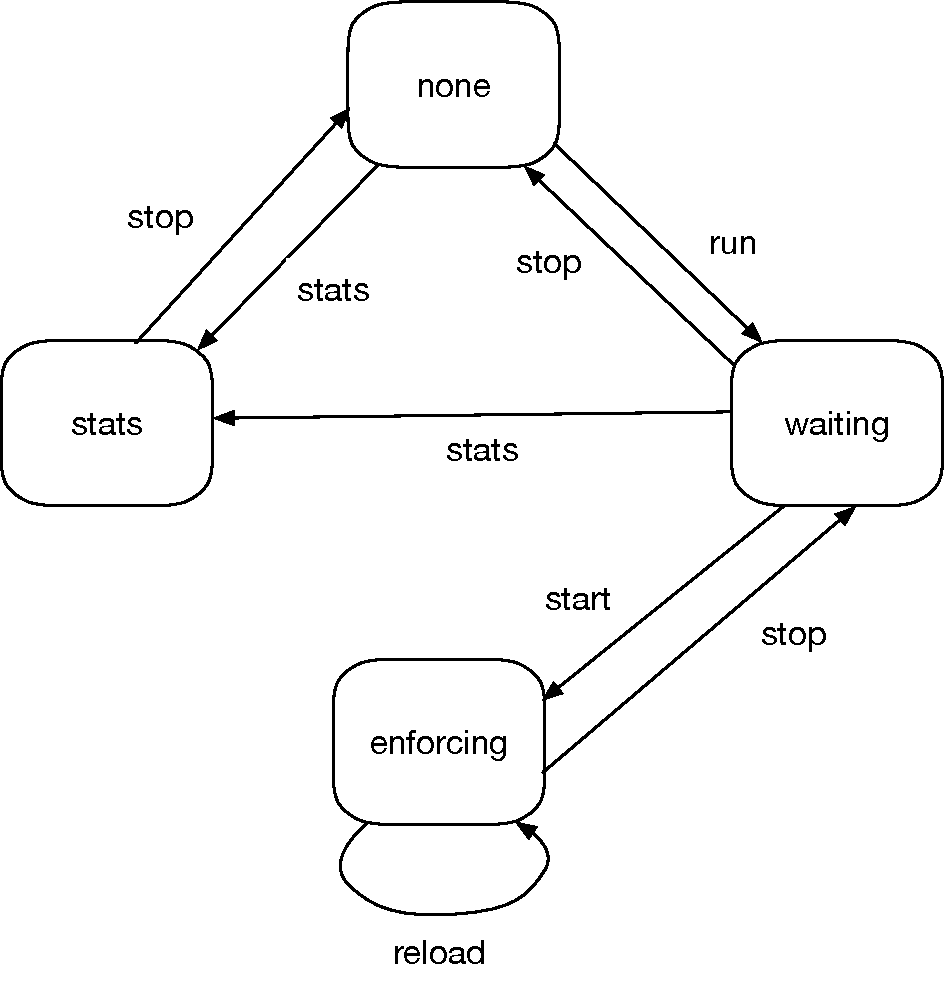
\includegraphics[width=.6\textwidth]{state_machine}
\caption{VpnService状态迁移图}\label{fig:3}
\end{figure}


\subsection{数据分析模块}
数据分析模块主要负责对文件描述符读写数据,该模块运行在一个native线程中,由VPN服务模块通过JNI调用启动。



\subsubsection{处理通信流量}

在我们的应用中,不需要创建一个到远程服务的隧道,但需要处理文件描述符中的数据。我们需要从文件描述符读取发送出来的流量,将其分析过滤,然后将其标记,然后写回文件描述符。这个过程使用C语言调用Android NDK API完成,然后通过JNI在Java代码中调用。首先,需要对文件描述符进行操作。

\subsubsection{文件描述符的操作}

文件描述符是一个用于表述指向文件的引用的抽象化概念。我们需要对Vpn创建后返回的文件描述符进行操作,从中读取数据包进行处理。我们采用epoll机制进行文件描述符的监听,以下为需要使用的函数:

\begin{lstlisting}[language=c]
int epoll_create(int size);//创建一个epoll文件,size用来告诉内核这个监听的数目一共有多大
int epoll_ctl(int epfd, int op, int fd, struct epoll_event *event);
int epoll_wait(int epfd, struct epoll_event * events, int max_events, int timeout);
\end{lstlisting}

\begin{enumerate}
	\item \lstinline {int epoll_create(int size); }
创建一个epoll的句柄,size用来告诉内核这个监听的数目一共有多大,参数size并不是限制了epoll所能监听的描述符最大个数,只是对内核初始分配内部数据结构的一个建议。当创建好epoll句柄后,它就会占用一个fd值,在linux下如果查看/proc/进程id/fd/,是能够看到这个fd的,所以在使用完epoll后,必须调用close()关闭,否则可能导致fd被耗尽。

	\item \lstinline {int epoll_ctl(int epfd, int op, int fd, struct epoll_event *event);}

函数是对指定描述符fd执行op操作。
	\begin{itemize}
		\item epfd:是epoll\_create()的返回值。\label{item:2}
		\item \verb|op:表示op操作,用三个宏来表示:添加EPOLL_CTL_ADD,删除EPOLL_CTL_DEL,修改EPOLL_CTL_MOD。分别添加、删除和修改对fd的监听事件。|
		\item fd:是需要监听的fd(文件描述符)
		\item epoll\_event:是告诉内核需要监听什么事,struct epoll\_event结构如下:
		\begin{lstlisting}[language=c]
struct epoll_event {
  __uint32_t events;  /* Epoll events */
  epoll_data_t data;  /* User data variable */
};
		\end{lstlisting}
	events可以是以下几个宏的集合:
		\begin{itemize}
			\item EPOLLIN :表示对应的文件描述符可以读(包括对端SOCKET正常关闭);\label{item:3}
			\item EPOLLOUT:表示对应的文件描述符可以写;
			\item EPOLLPRI:表示对应的文件描述符有紧急的数据可读(这里应该表示有带外数据到来);
			\item EPOLLERR:表示对应的文件描述符发生错误;
			\item EPOLLHUP:表示对应的文件描述符被挂断;
			\item EPOLLET: 将EPOLL设为边缘触发(Edge Triggered)模式,这是相对于水平触发(Level Triggered)来说的。
			\item EPOLLONESHOT:只监听一次事件,当监听完这次事件之后,如果还需要继续监听这个socket的话,需要再次把这个socket加入到EPOLL队列里
		\end{itemize}
	\end{itemize}
	\item \lstinline {int epoll_wait(int epfd, struct epoll_event *events, int max_events, int timeout);}
等待epfd上的io事件,最多返回max\_events个事件。

参数events用来从内核得到事件的集合,maxevents告之内核这个events有多大,这个maxevents的值不能大于创建\verb|epoll_create()|时的size,参数timeout是超时时间(毫秒,0会立即返回,-1将不确定,也有说法说是永久阻塞)。该函数返回需要处理的事件数目,如返回0表示已超时。

调用\verb|epoll_wait|时,线程会堵塞直至得到事件或者超时。其返回值i表示就绪的文件描述符的数目,当其大于0时,我们需要遍历events数组,数组里包含i个已经就绪的文件描述符。从就绪的文件描述符读取数据后进行解析和处理。
\end{enumerate}

\subsubsection{IP数据包处理}

%% http://www.ciscopress.com/articles/article.asp?p=348253&seqNum=4

从文件描述符读取的数据是IP数据包,IP数据包中包含了将数据在因特网上路由和传输的必要的信息,这部分信息存在于IP首部中
,对我们的应用格外重要的包括IP协议版本,源IP,目的IP等信息,我们需要实现对IP头的解析,以便于应用过滤规则。IP协议分为IPv4和IPv6,需要分别解析。

IPv4报文的首部包含13个必须字段,1个可选字段。所有字段均为大端的二进制顺序。IPv4首部结构如表\autoref{tab:1}所示。

\begin{table}[h!]
\centering
\caption{IPv4首部结构}\label{tab:1}
\begin{tabular}{|c|c|c|c|c|c|c|}
	\hline
	位偏移 & 0-3 & 4-7 & 8-13 & 14-15 & 16-18 & 19-31\\
	\hline
	0 & 版本 & 首部长度 & DSCP & 显式拥塞通告 & \multicolumn{2}{c|}{全长}\\
	\hline
	32 & \multicolumn{4}{c|}{标志符} & 标志 & 分片偏移 \\
	\hline
	64 & \multicolumn{2}{c|}{存活时间}& \multicolumn{2}{c|}{协议}& \multicolumn{2}{c|}{首部检验和} \\
	\hline
	96 & \multicolumn{6}{c|}{源IP地址} \\
	\hline
	128 & \multicolumn{6}{c|}{目的IP地址} \\
	\hline
	160 & \multicolumn{6}{c|}{选项(如首部长度>5)} \\
	\hline
	160 or 192+ & \multicolumn{6}{c|}{数据}\\
	\hline
\end{tabular}
\end{table}


其中值得我们关注的是:
\begin{table}[h!]
\begin{tabular}{l l}
	版本 & IP报文首部前4位是版本,我们需要对IPv4和IPv6采用不同的解析方式;\\
	首部长度(IHL) & 第二个字段是4位首部长度,说明首部有多少32位字长。\\
	协议 & 这个字段定义了该报文数据区使用的协议。IANA维护着一份协议列表(最初由RFC 790定义)。\\
	源地址 & 一个IPv4地址由四个字节共32位构成,此字段的值是将每个字节转为二进制并拼在一起所得到的32位值。\\
	目的地址 & 与源地址格式相同,但指出报文的接收端。
\end{tabular}
\end{table}


在netinet/ip.h头文件中定义了名为iphdr的结构体:
\begin{lstlisting}[language=c]
        struct iphdr {
        #if defined(__LITTLE_ENDIAN_BITFIELD)
            uint8_t  ihl    :4,
                 version:4;
        #elif defined (__BIG_ENDIAN_BITFIELD)
            uint8_t  version:4,
                 ihl    :4;
        #else
        #error	"Please fix <asm/byteorder.h>"
        #endif
            uint8_t	  tos;
            uint16_t  tot_len;
            uint16_t  id;
            uint16_t  frag_off;
            uint8_t   ttl;
            uint8_t   protocol;
            uint16_t  check;
            int32_t   saddr;
            int32_t   daddr;
        };
\end{lstlisting}

首先从pkt报文段中读取协议字段,源地址和目的地址:

\begin{lstlisting}[language=c]

        struct iphdr *ip4hdr = (struct iphdr *) pkt;

        protocol = ip4hdr->protocol;
        saddr = &ip4hdr->saddr;
        daddr = &ip4hdr->daddr;

\end{lstlisting}

还需要读取有效载荷的偏移位置payload:

\begin{lstlisting}[language=c]
         uint8_t ipoptlen = (uint8_t) ((ip4hdr->ihl - 5) * 4);
         payload = (uint8_t *) (pkt + sizeof(struct iphdr) + ipoptlen);
\end{lstlisting}

对于IPv6协议,我们需要有不同的处理方法,由于IPv6除了固定的首部(Fixed Header)存在多个扩展首部(Extension Header),所以获得载荷偏移位置较为复杂。下面为IPv6的Fiexed Header结构:


\begin{table}[h!]
\centering
\caption{IPv6固定首部结构}\label{tab:1}
\begin{tabular}{|c|c|c|c|c|c|c|}
	\hline
	位偏移 & 0-3 & 4-7 & 8-11 & 12-15 & 16-23 & 24-31\\
	\hline
	0 & 版本 & \multicolumn{2}{c|}{流量类} & \multicolumn{3}{c|}{流标签}\\
	\hline
	32 & \multicolumn{4}{c|}{负载长度} & 下一个首部的类型 & Hop限制 \\
	\hline
	64 & \multicolumn{6}{c|}{源IP地址} \\
	\hline
	192 & \multicolumn{6}{c|}{目的IP地址} \\
	\hline
\end{tabular}
\end{table}




IPv6的固定首部后,可能存在多个包含下层协议信息的扩展首部;可选的扩展首部后面才是包含上层协议信息的载荷。最后一个首部的Next Header中的值表示接下来的载荷是何种上层协议的信息,其他首部的Next Header表示下一个首部的类型。根据IPv6的相关标准,目前已经定义以下值的可选首部:



https://technet.microsoft.com/en-us/library/cc958821.aspx


\begin{lstlisting}[language=c]
        uint16_t off = 0;
        protocol = ip6hdr->ip6_nxt;
        if (!is_upper_layer(protocol)) {
            log_android(ANDROID_LOG_WARN, "IP6 extension %d", protocol);
            off = sizeof(struct ip6_hdr);
            struct ip6_ext *ext = (struct ip6_ext *) (pkt + off);
            while (is_lower_layer(ext->ip6e_nxt) && !is_upper_layer(protocol)) {
                protocol = ext->ip6e_nxt;
                log_android(ANDROID_LOG_WARN, "IP6 extension %d", protocol);

                off += (8 + ext->ip6e_len);
                ext = (struct ip6_ext *) (pkt + off);
            }
            if (!is_upper_layer(protocol)) {
                off = 0;
                protocol = ip6hdr->ip6_nxt;
                log_android(ANDROID_LOG_WARN, "IP6 final extension %d", protocol);
            }
        }
\end{lstlisting}

在完成IP层的IP首部的解析后,我们已经获知了数据包的源IP,目的IP,载荷偏移地址和传输层协议。根据协议的不同,我们还需进行进一步的解析。我们准备支持的传输层协议包括TCP,UDP,ICMP和ICMPv6协议。这些协议的值定义在linux/in.h文件中。下面我们需要对不同协议进行分别处理。

\subsubsection{TCP协议报文解析}

在IP首部中,协议字段值为6,即0x06时,该IP报文携带的数据为TCP协议的数据。TCP(Transmission Control Protocol )提供了点对点,面向连接的可靠传输服务。TCP负责建立TCP连接,在传输过程中,TCP有序发送数据报并进行确认,对丢失的数据报进行重发恢复。我们对TCP层的数据进行解析的主要目的包括两个:
    
    \begin{itemize}
       	\item 获知TCP数据报的来源端口和目的端口
       	\item 确定TCP连接握手建立和断开的时间,用以统计网络连接时长和发送的包的大小,为用户提供流量统计等功能
    \end{itemize}
    
TCP首部的结构如\autoref{tab:4}。

\begin{table}[h!]
\centering
\caption{TCP报文首部结构}\label{tab:4}
\begin{tabular}{|c|c|c|c|c|}
	\hline
	位偏移 & 0-3 & 4-7 & 8-15 & 16-31\\\hline
	0 & \multicolumn{3}{c|}{来源端口} & 目的连接端口 \\\hline
	32 & \multicolumn{4}{c|}{序列号码}  \\\hline
	64 & \multicolumn{4}{c|}{确认号码}  \\\hline
	96 & 报头长度 & 保留 & 标志符 & 窗口大小 \\	\hline
	128 & \multicolumn{3}{c|}{校验和} & 紧急指针 \\\hline
	160 & \multicolumn{4}{c|}{选项字段} \\\hline
	160 or 192+ & \multicolumn{4}{c|}{数据}\\\hline
\end{tabular}
\end{table}

TCP协议使用端口号进行区分发送方和接收方的应用层,我们需要实现对来源连接端口和目的连接端口进行解析读取。

如下代码可实现对端口的解析:

\begin{lstlisting}[language=c]
    char source[INET6_ADDRSTRLEN + 1];
    char dest[INET6_ADDRSTRLEN + 1];
    if (s->tcp.version == 4) {
        inet_ntop(AF_INET, &s->tcp.saddr.ip4, source, sizeof(source));
        inet_ntop(AF_INET, &s->tcp.daddr.ip4, dest, sizeof(dest));
    } else {
        inet_ntop(AF_INET6, &s->tcp.saddr.ip6, source, sizeof(source));
        inet_ntop(AF_INET6, &s->tcp.daddr.ip6, dest, sizeof(dest));
    }
\end{lstlisting}

对于TCP连接的建立和结束时间的监控过程较为复杂,需要对TCP连接的详细过程进行了解。

\subsubsection{TCP状态图}

TCP协议工作的过程包括三个部分:创建连接,数据传输和连接终止。这个过程中TCP连接的状态复杂,我们需要对其中的状态变化进行分析才能获知TCP连接传输的时间和数据信息。其状态图如图所示:
\todo{添加状态图}


\begin{itemize}
	\item LISTEN \\
 表示正在等待任一远程的TCP的连接
	\item SYN-SENT \\
 表示已经发送SYN请求之后,正在等待对应连接的SYN请求
	\item SYN-RECEIVED \\
 表示正在等待确认连接的请求,并且此时已经收到了SYN和发送了连接请求
	\item ESTANLISHED \\
 表示双方据已经建立了连接,已经可以开始传输数据了
	\item FIN-WAIT-1 \\
 表示等待远程TCP防的连接终止请求,或先前发送的连接终止请求的确认应答
	\item FIN-WAIT-2 \\
 表示等待远程TCP防的连接终止请求7.	4.1.2.3小节的代码加上适当注释。其他有代码的地方也是如此。
	\item CLOSE-WAIT \\
 表示等待本地用户的连接终止请求
	\item CLOSING \\
 表示等待远程TCP的连接终止请求的确认应答
	\item LAST-ACK \\
 表示等待先前发送给远程TCP的终止请求的确认应答
	\item TIME-WAIT \\
 表示等待过去足够的时间,确保远程TCP接收到了它发送的连接终止请求。MSL(maximum segment lifetime)用来表示TCP连接能在TIME-WAIT状态等待的最大时间,这个值的最大值为4分钟
	\item CLOSED \\
  表示目前没有任何连接状态
\end{itemize}

\subsubsection{TCP创建连接过程}



TCP在创建连接时,采用了三次握手。在客户端连接服务器之前,服务器必须首先绑定一个端口,打开此端口并监听连接,即被动打开。一旦进入这个状态,客户端就可以将状态转换为活跃打开。这三次握手的具体过程为:

\begin{enumerate}
	\item SYN \\ 客户端发送一个SYN报文到服务端,进入活跃打开状态。客户端设定一个随机的报文序列号A;
	\item SYN-ACK \\ 服务器返回一个SYN-ACK报文。这个报文的确认码设定为上一个SYN报文的序列号加1,即A+1,序列码是服务器设定的一个随机数B;
	\item ACK \\ 最后客户端发送ACK报文给服务器。该报文的序列号设定为A+1,确认码设定为上一个接收到的报文的序列码+1,即B+1.
\end{enumerate}

经过了上面的三次握手后,客户端和服务端均确认了全双工的连接。


\subsubsection{TCP创建连接终止过程}

TCP连接的终止过程,需要使用4次握手对两个方向连接分别终止。当一端想要终止一方的连接时,它需要发送一个FIN包,然后另一端发送ACK确认。所以终止TCP连接需要一对FIN和ACK报文。但也可以只使用三次握手终止,即在另一方发送ACK确认时,同时发送FIN终止另一方的连接。

\subsubsection{UDP协议的处理}
在IP首部中,协议字段值为17,即0x11时,该IP报文携带的数据为UDP协议的数据。UDP提供的是一种简单的无连接的传输模型。UDP提供了校验和用于检验数据完整性,提供了源端口和目的端口用于区别不同的地址的功能。UDP协议没有握手过程,提供的是不可靠的数据传输:不保证数据的传输成功,数据的有序和不排除重复。

    
UDP首部的结构如\autoref{tab:5}。

\begin{table}[h!]
\centering
\caption{UDP报文首部结构}\label{tab:5}
\begin{tabular}{|c|c|c|c|c|}
	\hline
	位偏移 & 0-7 & 8-15 & 16-23 & 24-31\\\hline
	0 & \multicolumn{2}{c|}{源端口} & \multicolumn{2}{c|}{目的端口} \\\hline
	32 & \multicolumn{2}{c|}{长度} & \multicolumn{2}{c|}{校验和} \\\hline
	\end{tabular}
\end{table}

UDP的首部由4个部分组成,长度均为16 bits,其中长度字段定义了UDP的头部和数据的总长度,单位为byte,最小长度为8,因为首部为8个byte。校验和字段用于检验UDP首部和数据段的错误,在IPv4中,这个字段是可选的,如果不使用,这个字段是全0,而在IPv6中,这个字段是必须的。

\subsection{防火墙规则模块}

由于支持多种特殊情况下的组合防火墙规则,防火墙规则较为复杂,在实现上设计了三类规则。
第一类规则是全局默认规则,该规则对全局生效,用于储存确定缺省行为,其字段如\autoref{tab:4-1-3-1}所示,这些字段全部为布尔变量类型,只允许true和false的值。


\begin{table}[h!]
	\centering
	\caption{全局默认规则字段表}\label{tab:4-1-3-1}
	\begin{tabular}{|c|c|c|c|}
		\hline
		字段名					&	字段类型		&	默认值	&	字段说明 \\\hline
		wifi\_default			& 	boolean 		& 	true	&	默认是否允许WIFI网络环境\\\hline
		other\_default 			& 	boolean 		& 	false	& 	默认是否允许其他网络环境\\\hline
		screen\_wifi\_default 		& 	boolean 		& 	false	&	亮屏时默认是否允许WIFI\\\hline
		screen\_other\_default 	& 	boolean 		& 	false	&	亮屏时默认是否允许其他网络环境\\\hline
		roaming\_default 			& 	boolean 		& 	false	&	默认是否允许漫游\\\hline
	\end{tabular}
\end{table}

第二类规则是应用特定规则,这种规则存在多条,每一条只对特定的应用生效,用于定义某个应用的所有流量的缺省行为,其字段如\autoref{tab:4-1-3-2}所示。这类规则采用info字段唯一标示一个应用,info中储存的是应用的UID,UID由系统定义。除info外,其他字段均为布尔变量,除了true和false,这些字段还允许为空,当这些字段为空时,防火墙拦截逻辑将会采用第一类全局默认规则中相应的字段的值。

\begin{table}[h!]
	\centering
	\caption{应用特定规则字段表}\label{tab:4-1-3-2}
	\begin{tabular}{|c|c|c|c|}
		\hline
		字段名			&	字段类型		&	默认值	&	字段说明 \\\hline
		info			&	long 		&	无		&	标识规则适用的应用的UID\\\hline
		wifi\_blocked	& 	boolean 		& 	null		&	WIFI网络环境下默认禁止\\\hline
		other\_blocked 	& 	boolean 		& 	null		& 	其他网络环境下默认禁止\\\hline
		screen\_wifi 	& 	boolean 		& 	null		&	亮屏时允许WIFI\\\hline
		screen\_other 	& 	boolean 		& 	null		&	亮屏时允许其他网络环境\\\hline
		roaming 		& 	boolean 		& 	null		&	允许漫游\\\hline
		apply	 		& 	boolean 		& 	true		&	规则是否启用\\\hline
	\end{tabular}
\end{table}

第三类规则是应用目的地址特定规则,这种规则不仅包含了应用的id的字段标明适用的包,还包含了目的host字段,标明适用的目的地址,字段如\autoref{tab:4-1-3-3} 。当某个流量存在该类规则适用时,将会优先采用这类规则,如果不存在适用规则,则会根据第二类规则处理,以此类推。

\begin{table}[h!]
	\centering
	\caption{应用目的地址特定规则字段表}\label{tab:4-1-3-3}
	\begin{tabular}{|c|c|c|c|}
		\hline
		字段名			&	字段类型		&	默认值	&	字段说明 \\\hline
		info			&	long 		&	无		&	标识规则适用的应用的UID\\\hline
		host			& 	string 		& 	无		&	目的host\\\hline
		block			&	boolean		&	无		& 	是否允许使用此规则的流量的访问\\\hline
	\end{tabular}
\end{table}

这三类规则的优先级是 应用目的地址特定规则 > 应用特定规则 > 全局默认规则。而在同一类规则中,存在多种网络环境,即是否漫游,是否亮屏,是否Wifi,这种网络环境的规则的优先级是 禁止漫游 > 亮屏允许 > 默认禁止。其具体的判断流程图如\autoref{fig:4-1-3-1}所示。

	\begin{figure}[h]
		\centering
		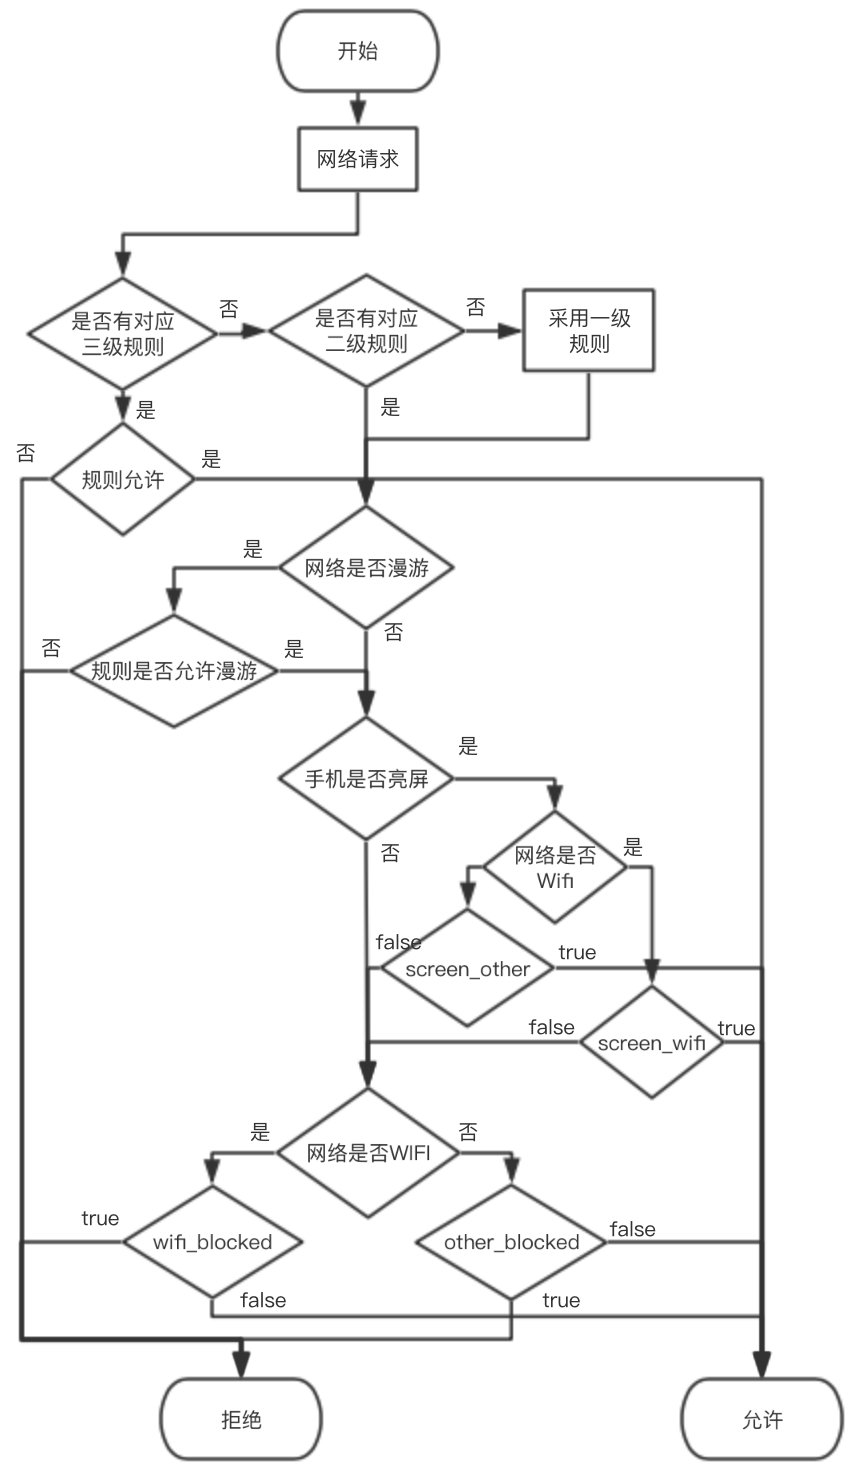
\includegraphics[width=0.8\textwidth]{process_4_1_rule.png}
		\caption{网络流量放行判断流程图}\label{fig:4-1-3-1}
	\end{figure}


	\FloatBarrier

	
\section{文件防护模块}

文件病毒防护由实时监控、自定义扫描、威胁处理和扫描记录四个功能组成,在代码实现上,将UI表现层和业务逻辑层分开,设计了如\autoref{fig:4-2}的逻辑架构。


\begin{figure}[!h]
	\centering
	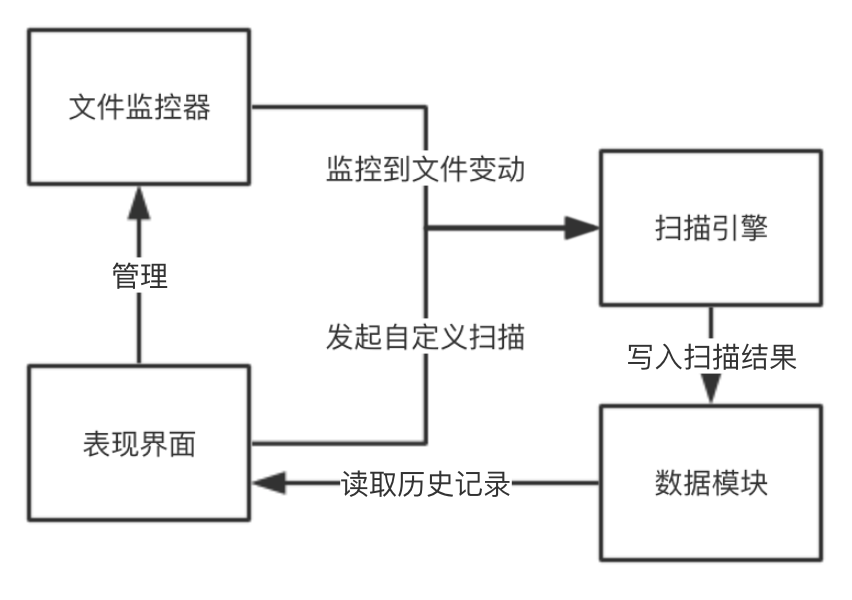
\includegraphics[width=.6\textwidth]{function_2_ori.png}
	\caption{文件防护架构图}\label{fig:4-2}
\end{figure}

这些模块的功能描述如下:

\begin{itemize}
    \item 表现模块\\ 表现模块主要是UI界面,包含对历史扫描记录的显示,威胁的处理,发起自定义扫描和配置文件监控扫描;历史记录和威胁处理主要和数据模块进行交互,发起扫描和配置文件监控则对扫描模块生效。
    \item 扫描模块\\ 扫描引擎FileScanService是一个Service,负责接收命令,扫描文件和发出扫描结果。FileScanService在HandlerThread中进行扫描,在UI Thread中进行消息接收和结果反馈。多线程之间通过Handler-Message机制进行交流,避免在主线程进行耗时操作; 
    \item 数据模块\\ 数据模块负责接收扫描模块的扫描结果,进行本地存储扫描记录。
\end{itemize}

\subsection{扫描模块}

扫描模块负责对文件的扫描,并且结果发出。其核心的逻辑如\autoref{fig:4-2-2}所示。

\begin{figure}[!h]
	\centering
	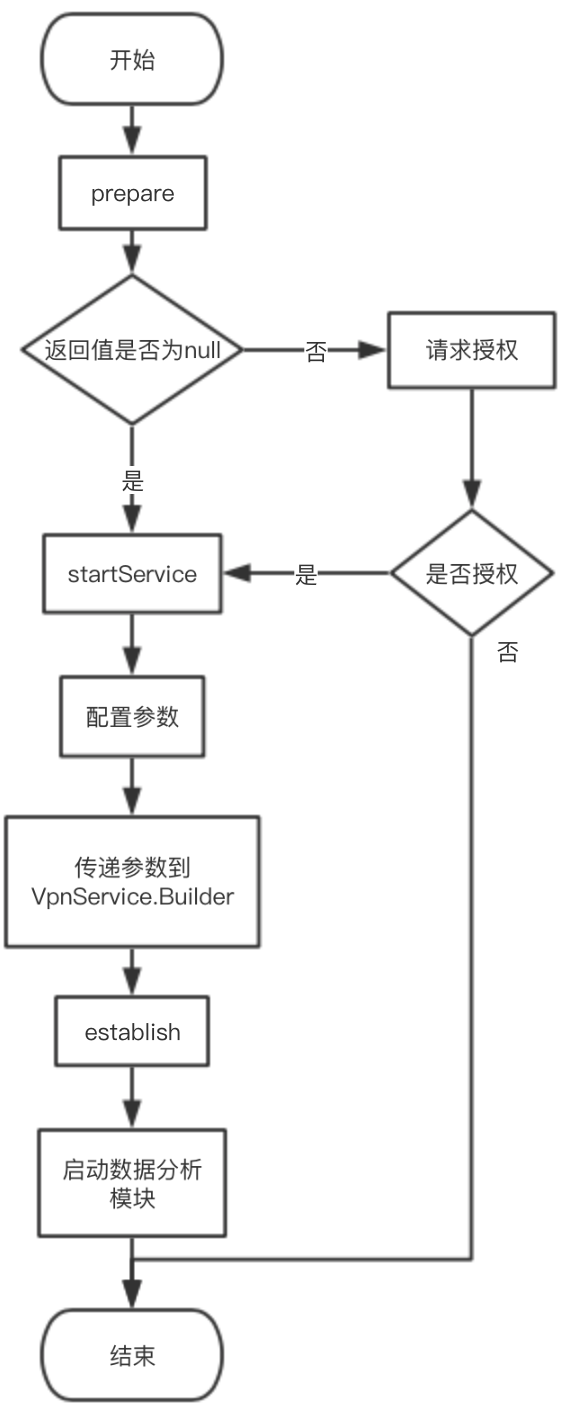
\includegraphics[width=.6\textwidth]{process_4_2_scan.png}
	\caption{扫描模块流程图}\label{fig:4-2-2}
\end{figure}

流程\autoref{fig:4-2-2}中 查询记录,上传文件,获取结果均需要网络请求。在这里我们采用了MetaDefender的云查杀API:
MetaDefneder的公开API需要通过HTTP协议进行请求,返回结果为json格式。我们需要对指定的url发起get或post请求,然后对返回的json字符串进行解析。

HASH查询是将可疑文件的哈希值作为参数查询历史扫描结果的快速扫描方式,该方式速度快,并且几乎不消耗通信流量。如果Hash查询无法到结果,则采用上传文件的方式发起扫描,发起扫描后需要查询扫描进度,当扫描完成时可以获得扫描结果。



\section{网页防护模块}


网页防护功能通过与防火墙协同工作实现,防火墙识别网页请求,并转发到网页防护进行处理。网页防护负责根据网页请求的URL进行查找本地黑名单,然后决定是否允许链接。

\begin{figure}[!h]
\centering
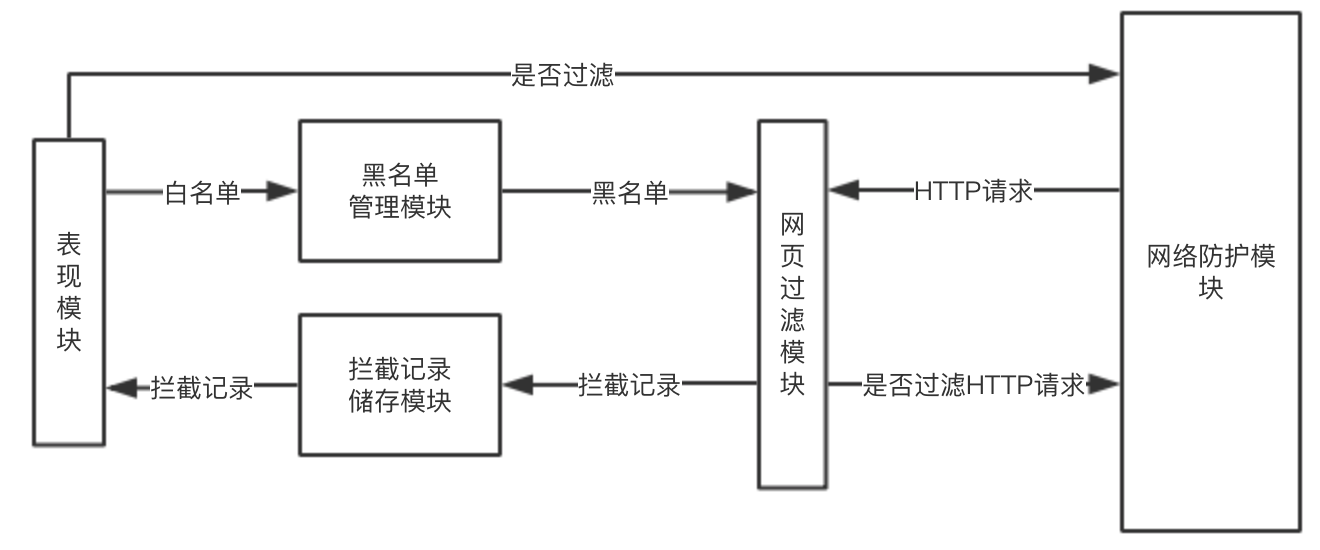
\includegraphics[width=1\textwidth]{function_3_ori.png}
\caption{网页防护架构图}\label{fig:4-3}
\end{figure}

\begin{itemize}
    \item 表现模块\\ 负责呈现UI界面,提供对网页防护的全局开关控制,对历史拦截记录的显示等
    \item 网络防护模块\\ 网络防护模块先前已经说明,它会在网络防护的过滤开关为开启状态时,将从所有流量中提取HTTP和HTTPS流量,将请求信息转发给网页过滤模块,并且根据网页过滤模块的返回结果决定数据包是否转发
    \item 网页过滤模块\\ 网页过滤模块负责从黑名单中匹配网页请求,并生成返回结果
    \item 黑名单管理模块\\ 黑名单模块负责提供剔除了用户定义的白名单的黑名单,并负责对名单定期更新
    \item 拦截记录储存模块\\ 负责存储拦截记录
\end{itemize}

\section{数据库持久化储存}

在本应用中,多种模块使用到了数据库持久化储存,数据模型及关系模式的设计在前面模块的设计中已经详细说明。本节主要针对在Android上进行数据库开发的一些技术实现进行介绍,包括数据库的连接和使用,数据库版本的维护等。

\subsection{Android SQLite}

   Android系统提供了SQLite数据库的支持,使用相关系统API即可实现数据库操作。对于操作数据库,需要实现如下一个类:

\begin{lstlisting}[language=java]
        public class DatabaseHelper extends SQLiteOpenHelper {

            @Override
            public void onCreate(SQLiteDatabase db) {
                Log.i(TAG, "Creating database " + DB_NAME + " version " + DB_VERSION);
                createTableLog(db);
                createTableAccess(db);
                createTableDns(db);
                createTableForward(db);
            }

            @Override
            public void onUpgrade(SQLiteDatabase db, int oldVersion, int newVersion) {

            }

        }
\end{lstlisting}

   该类用户每次打开数据库时,如果数据库表结构没有创建,会调用onCreate中相关代码进行创建表结构,如果数据库表版本不是最新,调用onUpgrade进行数据表版本的升级。
   打开数据库以后,可以进行数据库的读写操作。
   如下列代码可以实现从数据读取规则:

	\begin{lstlisting}[language=java]
        SQLiteDatabase db = this.getReadableDatabase();
        return db.query("access", null, "block >= 0", null, null, null, "uid");
	\end{lstlisting}

   下列代码更新了一条规则:

\begin{lstlisting}[language=java]
    lock.writeLock().lock();
    try {
        SQLiteDatabase db = this.getWritableDatabase();
        db.beginTransactionNonExclusive();
        try {
            ContentValues cv = new ContentValues();
            cv.put("allowed", packet.allowed ? 1 : 0);
            cv.put("uid", packet.uid);
            cv.put("version", packet.version);
            cv.put("protocol", packet.protocol);
            cv.put("daddr", dname == null ? packet.daddr : dname);
            cv.put("dport", packet.dport);

            rows = db.update("access", cv, "uid = ? AND version = ? AND protocol = ? AND daddr = ? AND dport = ?", new String[]{
                            Integer.toString(packet.uid),
                            Integer.toString(packet.version),
                            Integer.toString(packet.protocol),
                            dname == null ? packet.daddr : dname,
                            Integer.toString(packet.dport)});

            db.setTransactionSuccessful();
        } finally {
            db.endTransaction();
        }
    } finally {
        lock.writeLock().unlock();
    }
\end{lstlisting}

\subsection{ORM框架}

考虑到项目复杂,传统的数据库操作代码繁多,不易维护,我们决定使用ORM(Object-relational mapping)技术。ORM是一种将面向对象编程中的对象,和SQL数据库中的关系模式进行转换的技术。使用ORM技术后,更新对象模型,数据库关系模型也随之改变,不需要频繁更新修改SQL语句。避免人工撰写SQL语句也大大降低了出现bug的几率。

我们决定使用的ORM框架是OrmLite,这是一个轻量级的ORM框架实现,有针对Android优化的版本,效率高,易于使用。

	ORM框架直接将Java对象转换成相应的关系模式:Java对象每一种类存进一张表,将对象的成员变量转换为数据库中表的字段,java的基本类型会转换为数据库中相应类型,string会转换为varchar,使用Java注解可以添加其他约束条件,以及设置主键和索引。
	
	下面的代码实现了储存文件扫描结果到数据库:
	
	\begin{lstlisting}[language=java]
@DatabaseTable
public class Scan {
    @DatabaseField 
 	private Scan.Type type;
 	
    @DatabaseField
    public String path;

    @DatabaseField
    public String dataId;
    
    @DatabaseField
    public int inQueue = -1;
    
    @DatabaseField
    public String restIp;

    @DatabaseField
    public int scanAllResultI;
    
    @DatabaseField
    public int progressPercentage = -1;

    @DatabaseField
    public int totalAvs;

    @DatabaseField
    public int totalDetectedAvs;

    @DatabaseField
    public String displayName;

    @DatabaseField
    public String fileTypeExtension;
    
    @DatabaseField(id = true) 
    public long time = System.currentTimeMillis();
}
	\end{lstlisting}
	
	在上述代码中,类注解DatabaseTable标示这个类会存为数据库中的一张表,这个注解接受name参数,指明所存的表的表明,默认采用类名Scan;
	注解DatabaseField修饰的成员变量会作为表中的字段存入数据,没有这个注解的将会被忽略;这个注解接收多种参数,布尔类型id决定这个变量会被作为主键,布尔类型canBeNull来添加实体完整性的非null约束,还有index,unique等参数。
	
	在读写数据库时,需要使用到DAO类,这个类由ORMDatabaseHelper获得,如下代码获得了一个可以读写Scan的DAO类,并读出了Scan表中全部的行:
	\begin{lstlisting}[language=java]
	try{
		ORMDatabaseHelper helper = new ORMDatabaseHelper(this);
		Dao<Scan, Long> dao = mDatabaseHelper.getDao(Scan.class);
		List<Scan> scans = dao.queryForAll();
	} catch (SQLException e) {
		Log.e(TAG, "SQLException when query scan");
	}
	\end{lstlisting}
	
	DAO是用来读写数据库,刷新对象状态的,它包含了很多方法用于操作数据库,可以实现增删查改。
	\begin{lstlisting}[language=java]
		Scan target = new Scan();
		target.type = Danger;
		// 增		
		dao.create(target);
		// 改
		target.path = "/sdcard/Downloads/test.file";
		dao.update(target);
		// 查
		Scan result = dao.queryForFirst(target);
		List<Scan> results = dao.queryForMatching(target);
		// 删
		dao.delete(scan);	
	\end{lstlisting}

\section{轻量级持久化储存}

\subsection{序列化与文件}

和常规Java一样,Android中也可使用文件进行储存数据。如下面的代码将二进制数据写进了文件。

\begin{lstlisting}
byte data[] = ...
FileOutputStream out = new FileOutputStream("/sdcard/Android/log");
out.write(data);
out.close();
\end{lstlisting}

Java中允许将一个对象直接写入文件,此时需要使这个类实现Serializable接口,这个接口不包含任何需要实现的方法,只是用于标记。

\begin{lstlisting}
		FileOutputStream fout = new FileOutputStream("/sdcard/Android/log");
		ObjectOutputStream oos = new ObjectOutputStream(fout);
		oos.writeObject(address);
\end{lstlisting}

在我们的应用中,在配置导入导出,日志储存这些功能里,均采用文件的方式进行持久化储存。


\subsection{SharePreference储存}

除了防火墙规则,应用还需要储存一些状态信息,这些信息量少,也难以提取关系模型,比如VPN是否启用,用户是否在应用市场为我们的应用评过分,我们需要采取一些轻量级非关系型的存储方案。

SharePreference是Android系统提供的一种简单的Key-Value持久化机制。广泛用于储存应用配置。它在实现上创建了一个XML文件用来储存Key-Value,储存位置根据SharePreference是否私有来定,如果是私有的,将会储存在应用程序自己的沙箱中,无法被其他应用访问。具体使用方式如下:

如下代码会打开默认的SharePreference储存空间,并从中读取信息:

\begin{lstlisting}[language=java]
    final SharedPreferences prefs = PreferenceManager.getDefaultSharedPreferences(this);
    boolean enabled = prefs.getBoolean("enabled", false);
    boolean default_wifi = prefs.getBoolean("whitelist_wifi", true);
    boolean default_other = prefs.getBoolean("whitelist_other", true);
\end{lstlisting}

以下代码可以储入信息:

\begin{lstlisting}[language=java]
    final Editor editor = prefs.edit();
    editor.putBoolean("enabled", true);
    editor.putString("user_name","Carlos");
    editor.commit();
\end{lstlisting}

\section{兼容性}

\subsection{权限兼容}
Android系统要求应用软件对使用的权限进行声明,我们的安全应用使用到了网络,访问网络、WIFI、手机状态,在系统启动时自动启动,防止设备休眠,震动,访问文件系统这些权限。对此我们使用了如下声明:

\begin{lstlisting}[language=xml]
    <uses-permission android:name="android.permission.ACCESS_NETWORK_STATE"/>
    <uses-permission android:name="android.permission.READ_PHONE_STATE"/>
    <uses-permission android:name="android.permission.ACCESS_WIFI_STATE"/>
    <uses-permission android:name="android.permission.RECEIVE_BOOT_COMPLETED"/>
    <uses-permission android:name="android.permission.WAKE_LOCK"/>
    <uses-permission android:name="com.android.vending.BILLING"/>
    <uses-permission android:name="android.permission.INTERNET"/>
    <uses-permission android:name="android.permission.VIBRATE"/>
    <uses-permission android:name="android.permission.WRITE_EXTERNAL_STORAGE" />
\end{lstlisting}


在Android 5.1(API级别22)或更低版本的Android系统上,或者应用程序的targetSdkVersion为22或更低版本,在应用的Manifset文件作出上述权限声明,即可保证运行时已经被授予了上述权限,这些权限会在安装时被一次性授予,并且只能通过卸载应用来撤销。 但在6.0 (API级别23)或更高版本的Android系统上,应用程序需要在运行时请求用户的权限。 用户可以随时撤销权限,因此应用程序需要检查每次运行时是否具有权限。
对此,我们在是现实,对于需要权限的地方,均做了以下处理:
\begin{enumerate}
	\item 每次运行时检查权限是否满足
	\item 不满足权限要求时,要求用户授予权限
\end{enumerate}

\subsection{多尺寸屏幕显示兼容}


Android运行在多种多样的设备上,包括手机、平板电脑甚至电视机。这些设备的屏幕尺寸变化多样,即便仅仅定位于手机用户,手机屏幕尺寸和分辨率尺寸仍然千变万化,不同的手机屏幕尺寸为手机应用的兼容性提出了挑战。

针对多种屏幕尺寸和分辨率大小,首先需要提出像素密度的概念:像素密度指的是单位物理面积上屏幕的像素的多少。屏幕具有物理大小和分辨率两个关键指标,为了保证用户能够触摸和看清界面,文字、按钮等界面元素不能单一的根据屏幕的物理尺寸或分辨率来决定。现在的最新的手机屏幕保持着5寸左右的小屏幕,却有着胜过巨大屏幕的电视机屏幕的分辨率。总的来说,同样的物理大小的屏幕上,分辨率越高,单个文字或界面空间就应该占用更多的像素以保持相对不变的物理显示大小。

Android系统中提供了像素密度独立的尺寸单位,包括用于描述界面控件大小的dp单位和描述文字大小的sp单位,它们会自动地根据屏幕的像素密度选取合适的像素的尺度。所以在我们的UI界面开发中,广泛地使用了dp和sp作为尺寸单位。例如,使用如下代码可以创建一个ImageView,它的尺寸32dp,在不同的像素密度的屏幕上会采用合适的倍率。

\begin{lstlisting}
<ImageView
	android:layout_width="32dp"
	android:layout_height="32dp"
	android:layout_gravity="center_vertical"
	android:src="@mipmap/ic_launcher"/>
\end{lstlisting}

另外,相应的,我们还需要针对不同像素密度的屏幕使用不同尺寸的图像等资源文件。Android系统将手机密度分为lhdpi, mhdpi, hdpi, xhdpi, xxhdpi, xxhdpi,所以在使用drawable类资源时,放入带有此类后缀的资源文件夹中,使用时,手机就会更根据自身的像素密度选取合适的文件夹中的资源,例如在drawable-lhdpi和drawable-mhdpi中分别放入不同尺寸的名为icon.png的图片,在lhdpi的手机上,将会读取并使用drawable-lhdpi中的icon.png,而mhdpi的手机将会使用后者。以此,我们可以为不同手机提供合适的大小的图片。

\subsection{多版本API兼容}

Android系统由于代码开源,存在多种多样的定制版本,不同国家不同地区,用户使用的Android版本存在很多差异。这些差异不仅仅体现在UI界面上,也会在系统框架和系统API上广泛体现。Android这种版本过于零碎,操作系统体验极度分化的现象叫做碎片化。
Android碎片化,对我们开发Android应用带来了难度,实现一样功能,在不同的版本的Android系统上可能需要不同的应对的措施。我们集中解决Android SDK版本不一致带来的兼容性问题。
目前Android最新版本是Android7.1.2, 我们的应用计划支持Android 4.0及以上版本。对此,我们采用了如下措施来解决不同SDK版本存在的API差异的问题:

\subsubsection{SDK版本检查}
在一些情况下,我们需要在不同的SDK版本上调用不同的方法或者不同的参数,往往通过API检查来进行,如下代码在系统版本大于等于N和小于N时调用了不同的代码:
 
\begin{lstlisting}[language=java]
if (Build.VERSION.SDK_INT >= Build.VERSION_CODES.N)
  	builder.setContentTitle(getString(R.string.msg_started));
else
    builder.setContentTitle(getString(R.string.entry_firewall)).setContentText(getString(R.string.msg_started));
\end{lstlisting}


这类往往是用在,不同版本的API更换了类似功能的方法名和参数;仅仅在特定版本API才执行的操作;在更高版本有更佳的替代API等情况。

\subsubsection{兼容support包的使用}

某一些在更新版本的Android系统上所提供的新功能或者API,由于广泛在旧版本的Android上存在大量需求,Google提供了一系列的support兼容包来提供向后兼容,这些support包提供了新特性在旧版本的系统上的实现,使得开发者可以在旧版本系统上使用一些新版本上才有的功能和API。

在我们的应用中广泛使用了一些support依赖库:
\begin{itemize}
	\item appcompat \\ 这个support包提供了ActionBar的向下兼容实现,
	\item design\\ 这个support提供了Android 5.0新增的Material Design设计语言的向下兼容实现,使得Android 4.0~ Android 4.4的设备上可以实现Material Design视觉效果,从而让用户获得一致的视觉体验。
\end{itemize}

\subsubsection{自行封装多版本实现}

除了上述的兼容措施之外,仍然存在一些情况兼容性问题难以解决。例如在新版本的Android中支持图标的颜色滤镜,能够通过简单的代码,使得图片被处理成特定的颜色来显示;由此,我们自己设计实现了简单工具,其实现通过判断系统版本,在高级版本时直接使用系统自带的实现,而在低级版本自行实现图标颜色的处理。

\chapter{系统测试}

\section{兼容测试}

\subsection{测试项目}

\begin{enumerate}
	\item 在Android 5.1以下系统运行正常
	\item 在Android 6.0以上能提醒用户授权
	\item 在不同尺寸的屏幕上显示正常
\end{enumerate}

\subsection{测试结果}
\todo[inline]{更新7.0权限测试的图片}

\begin{enumerate}
	\item 在Android 5.1以下系统运行正常\\ 
在测试时,我们选取了Android 4.4的系统进行了权限测试,Android 4.4系统在安装时进行了权限授权,并且通过卸载app之外的方式无法撤销,程序运行正常。如\autoref{fig:5-1-1}。

	\begin{figure}[!h]
		\centering
		\includegraphics[width=0.3\textwidth]{test_5_1_1.png}
		\caption{Android 5.0权限测试}\label{fig:5-1-1}
	\end{figure}
	
	\item 在Android 6.0以上能提醒用户授权
在测试时,我们选取了Android 7.0的系统进行了权限测试,Android  7.0系统除了在安装时进行权限授权,还有一部分权限必须在运行时授权,我们的程序如期工作,如\autoref{fig:5-1-2}。
	\begin{figure}[!h]
		\centering
		\includegraphics[width=0.3\textwidth]{test_5_1_2.png}
		\caption{Android 7.0权限测试}\label{fig:5-1-2}
	\end{figure}
	
	\item 在不同尺寸的屏幕上显示正常
我们在不同尺寸和分辨率的屏幕上进行了测试,最小到480*800,最大为1440*2560,均能正常显示,并且用户操作较为方便。如\autoref{fig:5-1-3-0}是在1440*2560的屏幕上测试的显示,该手机屏幕像素密度是560dpi;\autoref{fig:5-1-3-1}是在分辨率480*800的手机上测试的显示,像素密度为hdpi。

\begin{figure}[!htb]
\centering
\minipage{0.32\textwidth}
	\includegraphics[width=\linewidth]{test_5_1_3_0.png}
	\caption{560dpi显示测试}\label{fig:5-1-3-0}
\endminipage
\hspace{1cm}
\minipage{0.32\textwidth}
	\includegraphics[width=\linewidth]{test_5_1_3_1.png}
	\caption{hdpi显示测试}\label{fig:5-1-3-1}
\endminipage
\end{figure}
	
\end{enumerate}

\section{功能测试}

\subsection{网络防护测试}

网络防护旨在提供传统防火墙的网络连接的管理功能,该功能要求能有效拦截应用的通信流量,阻止未授权的访问。如\autoref{fig:5_2_1}是测试网络防护的过程,首先在开启网络防护功能之后,会在通知栏显示通知,这显示应用的功能开启成功;然后在规则编辑界面将chrome应用的数据流量禁止,此时如果chrome无法在数据流量下访问网络,则说明测试成功;最后一张图显示任何chrome的网页请求均会无法访问,说明测试成功。

\FloatBarrier
	\begin{figure}
		\includegraphics[width=0.3\textwidth]{test_5_2_1_0.png}
	\hspace{0.3cm}
		\includegraphics[width=0.3\textwidth]{test_5_2_1_2.png}
	\hspace{0.3cm}
		\includegraphics[width=0.3\textwidth]{test_5_2_1_3.png}	
	\caption{网络防护测试}\label{fig:5_2_1}
\end{figure}
\FloatBarrier
	
\subsection{文件防护测试}

文件防护主要提供本地文件的实时文件系统监控扫描的功能,需要能监视文件系统的变动,进行扫描。测试时,首先需要开启该功能,然后下载任意文件,查看界面或通知里是否检测到了文件,并进行了查杀。如\autoref{fig:5_2_2},我们可以看到文件防护监视到了文件变动,并自动进行了扫描。

\FloatBarrier
	\begin{figure}[!h]
		\centering
		\includegraphics[width=0.3\textwidth]{5_2_2_0.png}
	\hspace{0.3cm}
		\includegraphics[width=0.3\textwidth]{5_2_2_1.png}
		\caption{文件防护测试}\label{fig:5_2_2}
	\end{figure}
\FloatBarrier

\subsection{网页防护测试}



\section{性能测试}


\chapter{结论}

在本文中,我们通过实现VPNService的方式,将Android系统的流量进行过滤和解析,通过自定义的个性化规则,实现了一种基于Android的网络防火墙。这个防火墙不仅具有传统防火墙根据通信的源地址和目的地址过滤拦截的功能,还针对移动互联网流量价格昂贵的环境,支持了WiFI和移动数据网络的区分,也支持漫游网络的区分;针对移动设备电能有限,存在延长电池续航的需求的特性,支持了亮屏下采用特殊规则。与传统防火墙往往面对的是专业网络管理员不同,我们针对专业技能较为有限的用户进行了优化:首先提供了友好而美观的图形交互界面,完善的使用提示;其次我们对规则的添加采取了交互式的方式,通过记录应用的网络请求,来让用户方便和有效的设置特定目的地址的屏蔽规则,也提供了whois等快捷工具性操作;最后我们为方便用户切换防火墙状态,也提供了快捷方式、通知栏控件等方式管理防火墙。除了实现流量的过滤以及管理,我们的网络防火墙对文件下载操作也提供了反病毒保护,我们支持对文件系统敏感区域进行监控保护,对可疑文件进行云端病毒扫描,实现发现可疑文件对用户进行提醒警报。在网页浏览方面,我们实现了不良网页的拦截,针对存在恶意代码的网站,进行屏蔽,保障安全。

我们对本论文实现的应用进行了测试,从兼容性,功能性和性能三个方面对应用软件进行了评估测试。在兼容性上,对权限系统进行了兼容,保证从Android 4.0到Android 7.1的广泛兼容,对不同尺寸的手机屏幕也提供了支持,绘制了不同高清程度的图片,使得应用软件在不同分辨率的屏幕上保持高可用;在功能性上,对我们在需求分析中提出的三大块功能进行了测试,确保功能都能正常使用和工作;在性能上,对手机的性能占用进行了评估,保证对用户手机的性能和续航的影响在可以接受的范围之内
总的来说,这篇论文从需求分析出发,进行了Android网络防火墙实现的概要分析,具体地阐述了网络防火墙应用的功能模块和软件架构,最后确认了Android网络防火墙在实际用户环境中的可行性和可用性,对本文提出的应用实现的架构的正确性和可行性提供了证明。


\backmatter


\bibliography{ref-example}


\end{document}
\endinput